\newpage 
\section{Understanding RPCs \& Synchronization with Go}
This section will cover the concept of Remote Procedure Calls (RPCs) and how they are used in distributed systems and use the Go programming language to demonstrate such.
\subsection{Establishing a Client-Server Connection}




\begin{Def}[client-server model]

    The client-server model is a distributed application structure that partitions tasks or workloads between the providers of a
     resource or service, \textbf{called servers}, and service requesters, \textbf{called clients}. 
     
     Often clients and servers communicate over a computer network on separate hardware, but both client and server may reside in the same system.

\end{Def}

\begin{Def}[Remote Procedure Call (RPC)]

    A Remote Procedure Call (RPC) is a protocol that allows a \textbf{client} computer request the execution of functions on a separate \textbf{server} computer.

    RPC's abstract the network communication between the client and server enabling developers to write programs that may run on different machines, but appear to run locally.
\end{Def}

\begin{Def}[RPC Call Stack]

    The RPC call stack facilitates communication between two systems via four layers:
    
    \begin{enumerate}
        \item \textbf{Application Layer:} The highest layer where the client application initiates a function call. On the server side, this layer corresponds to the service handling the request.
        
        \item \textbf{Stub:} A client-side stub acts as a proxy for the remote function, \textbf{marshaling arguments} (converting them into a transmittable format) and forwarding them to the RPC library. On the server side,
        a corresponding stub, \textbf{the dispatcher}, receives the request, unmarshals the data, and passes it to the actual function.
        
        \item \textbf{RPC Library:} The RPC runtime that manages communication between the client and server, ensuring request formatting, serialization, and deserialization.
        
        \item \textbf{OS \& Networking Layer:} The lowest layer, responsible for transmitting RPC request and response messages over the network using underlying transport protocols.
    \end{enumerate}
    
    The request message travels from the client's application layer down through the stack and across the network to the server. The server processes the request in reverse, executing the function and returning the result to the client.
\end{Def}
    
\newpage 

\noindent
To illustrate the RPC call stack, observe the following diagram:
\begin{figure}[h]
    \centering
    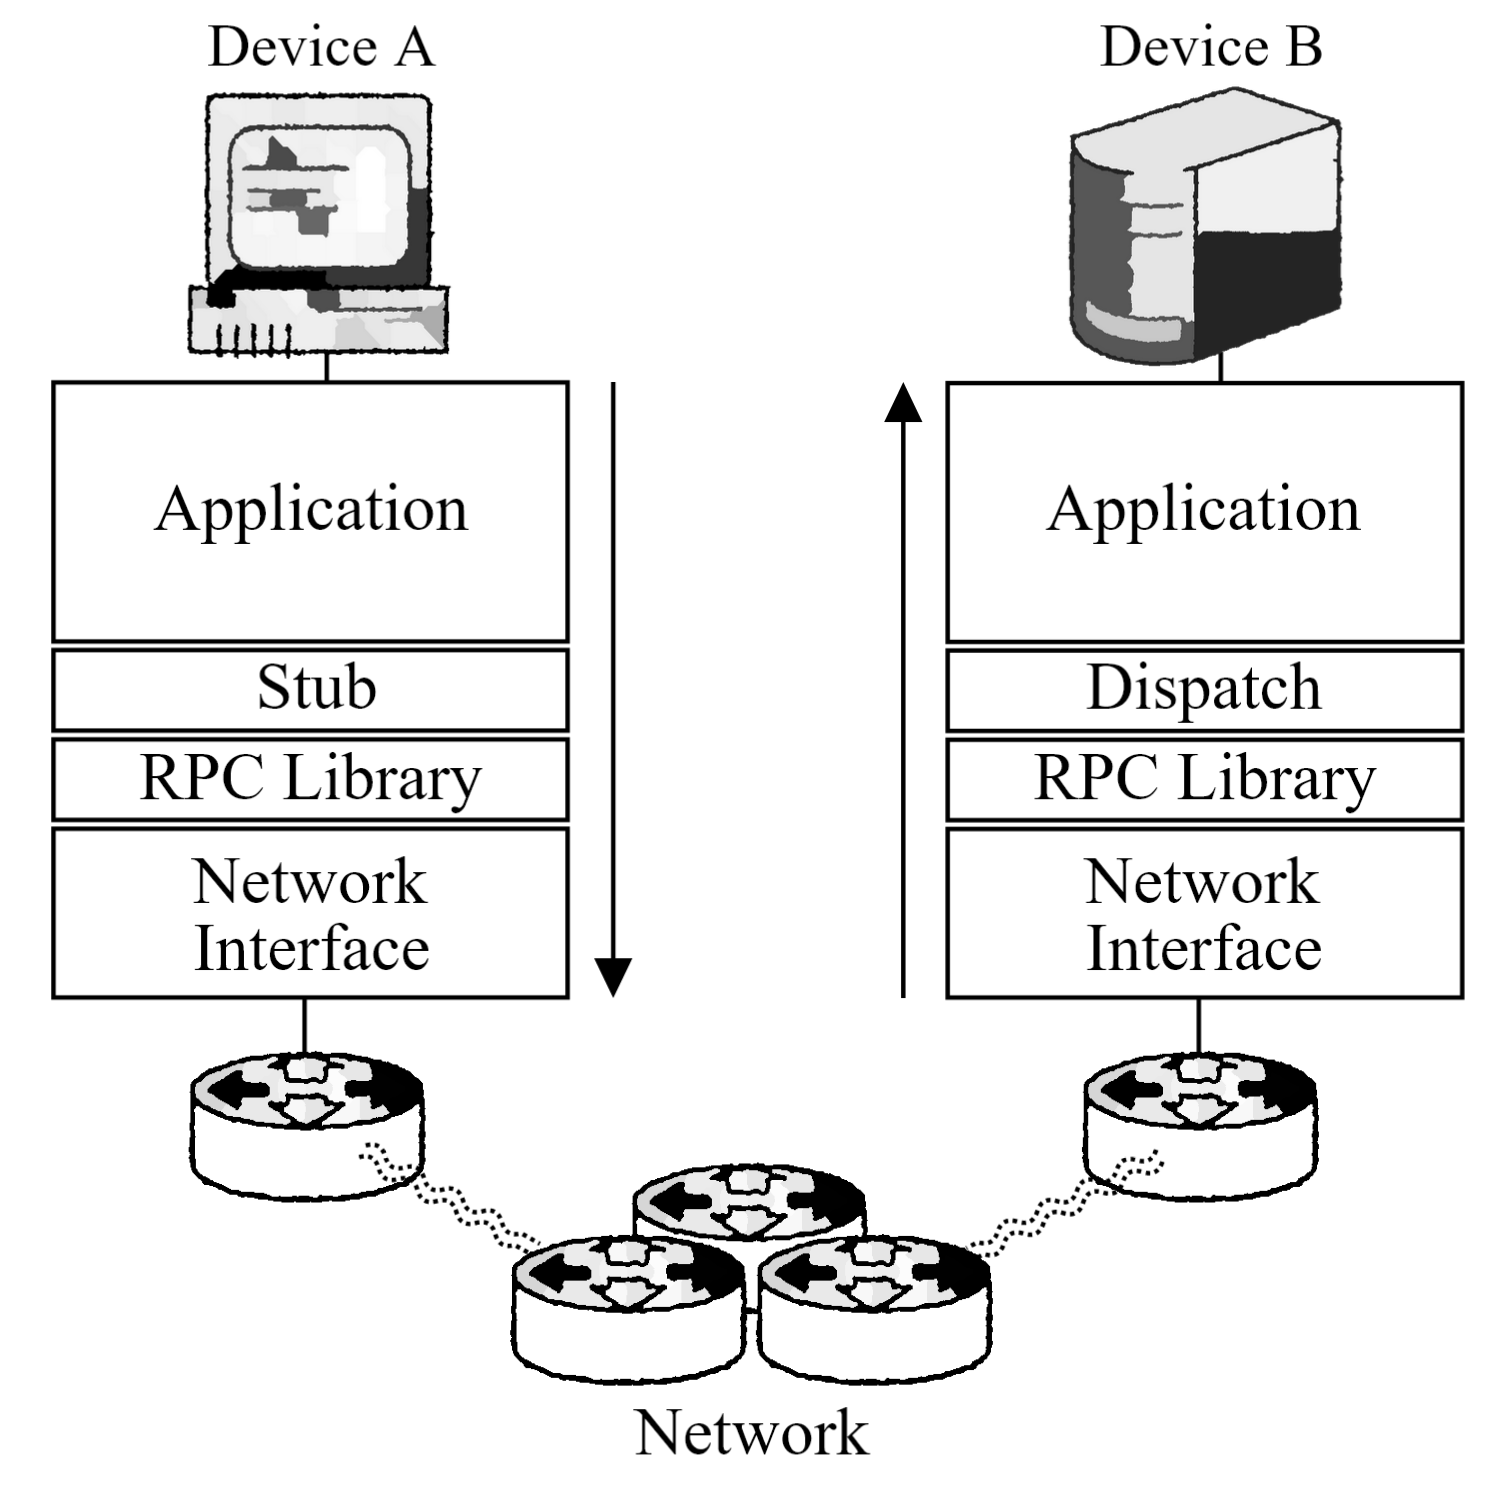
\includegraphics[width=0.55\textwidth]{Sections/rpc/rpc_stack.png}
    \caption{Client system $A$ making a request to Server system $B$ over RPC. This of which is 
    reciprocated by $B$ to return the result.}
    \label{fig:rpc_stack}
\end{figure}

\begin{figure}[h]
    \centering
    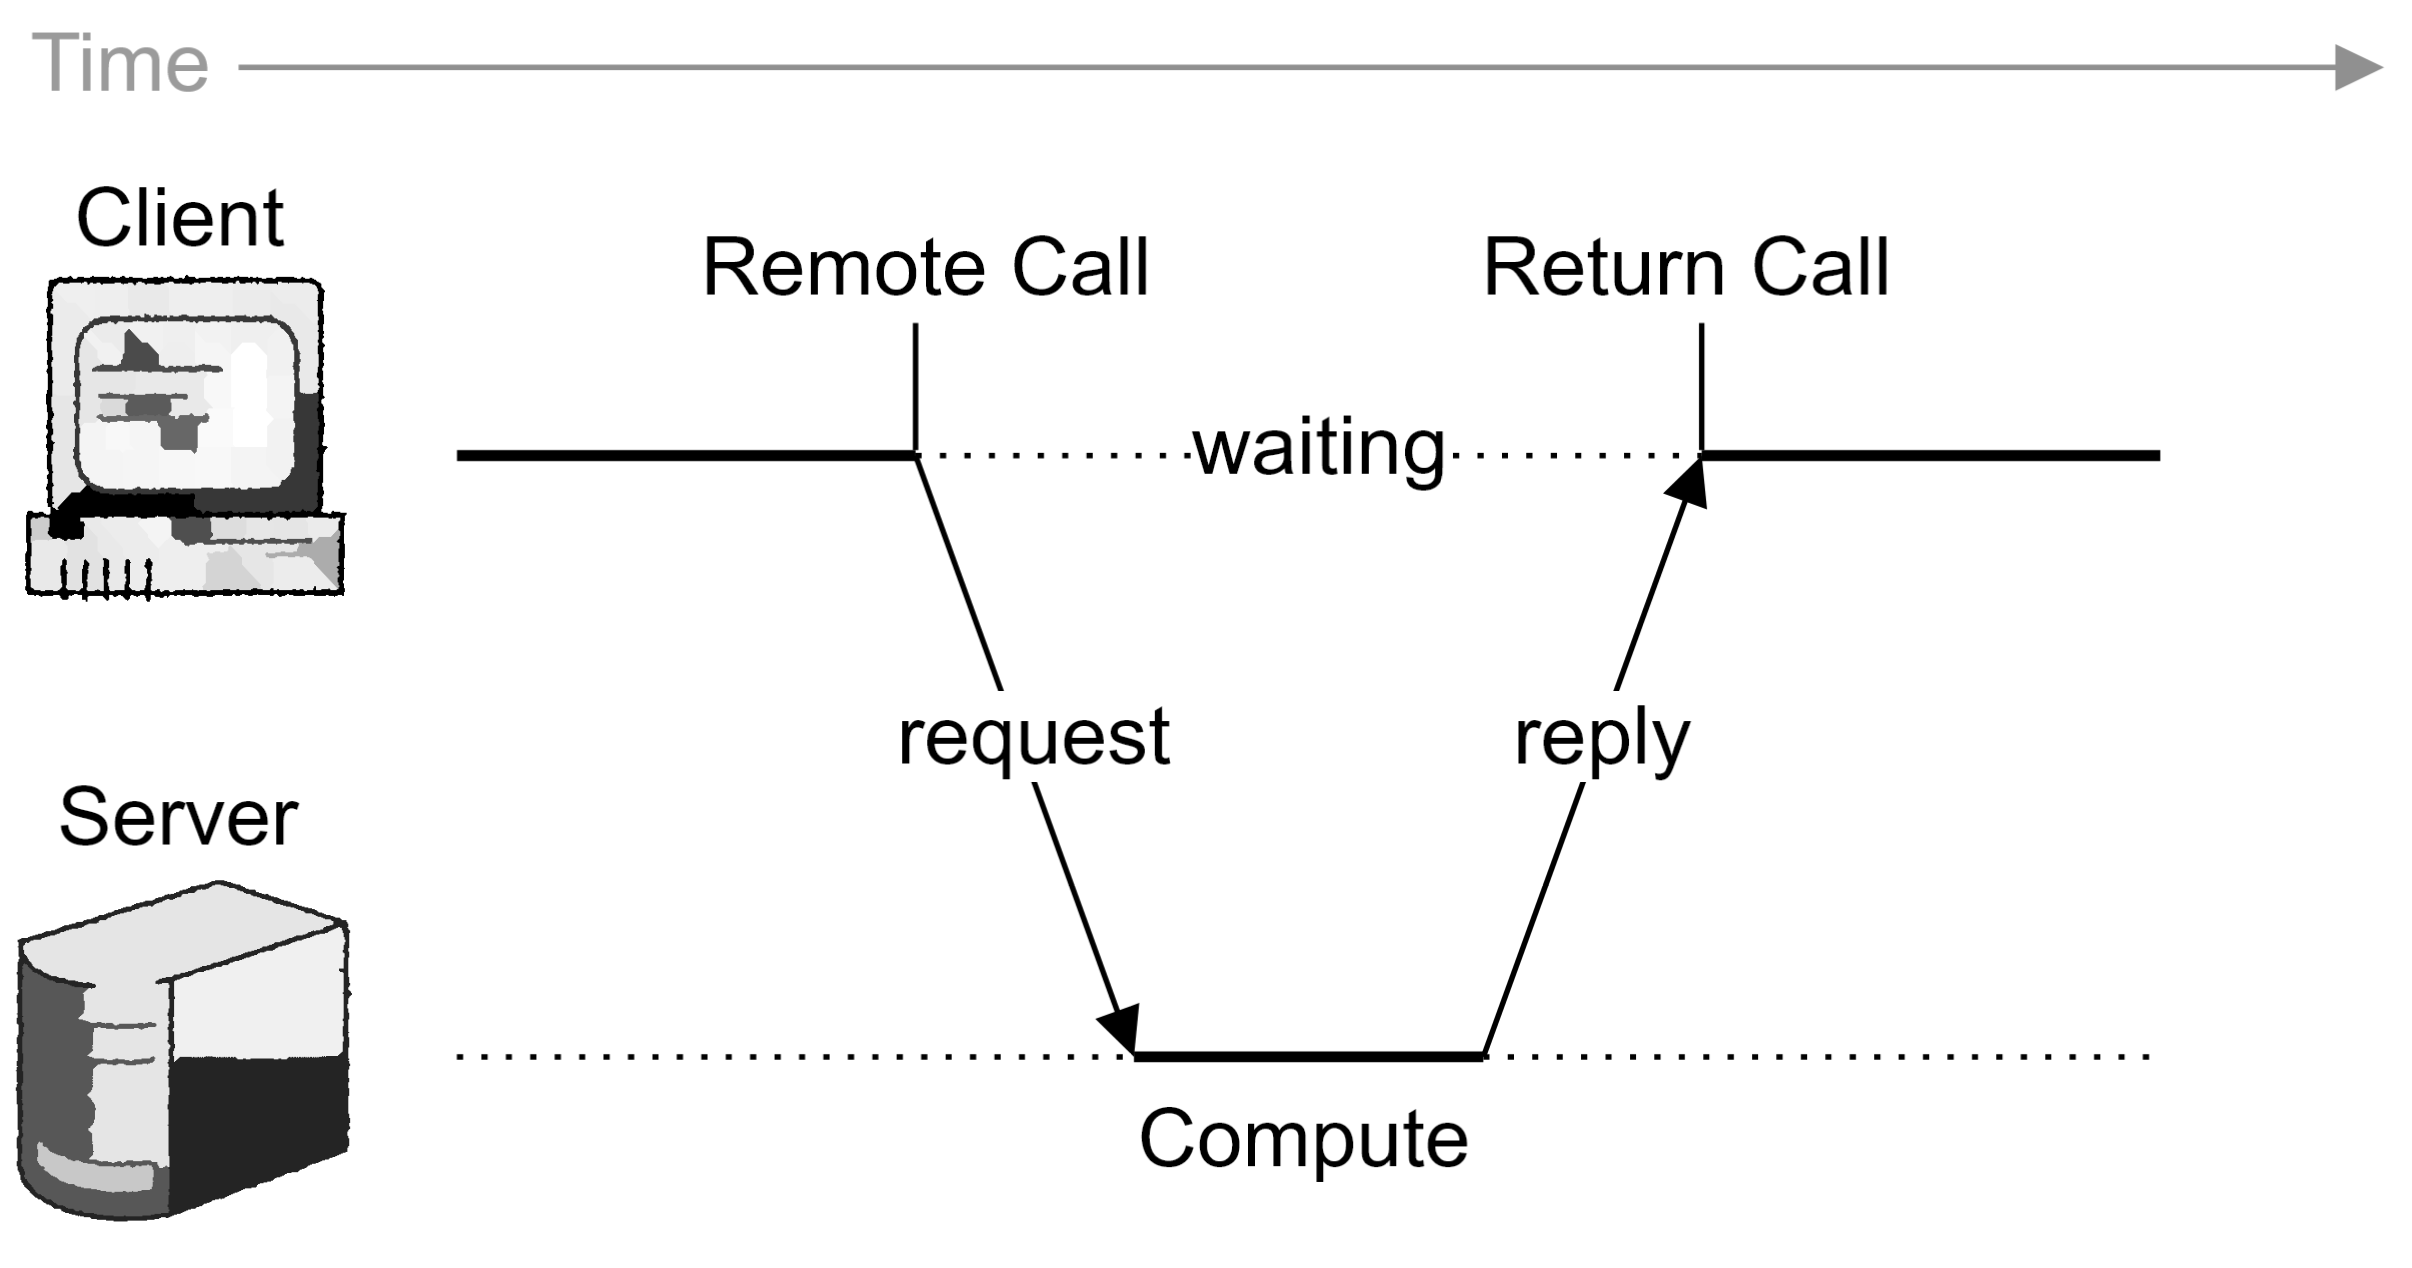
\includegraphics[width=0.63\textwidth]{Sections/rpc/call_time.png}
    
    \vspace{1em}
    \caption{RPC call stack over time. Once the client makes the call it waits for the server to process the request and return the result. The programmer need not worry beyond sending the request and receiving the response.
    The RPC deals with all the heavy work of facilitating the communication.
    }
    \label{fig:rpc_time}
\end{figure}

\newpage 

\noindent
Now to discuss what marshaling and unmarshaling are:
\begin{Def}[Marshaling and Unmarshaling]

    \textbf{Marshaling} handles data format conversions, converting the object into a byte stream (binary data).
    This conversion is known as \textbf{serialization}. This is done as the network can only transmit bytes\\
    
    \noindent
    \textbf{Unmarshaling} is the process of converting the byte stream into the original, object called \textbf{deserialization}. 
    This allows the server to process the request.
\end{Def}

\noindent
To illustrate serialization and deserialization, consider the following diagram:
\begin{figure}[h]
    \centering
    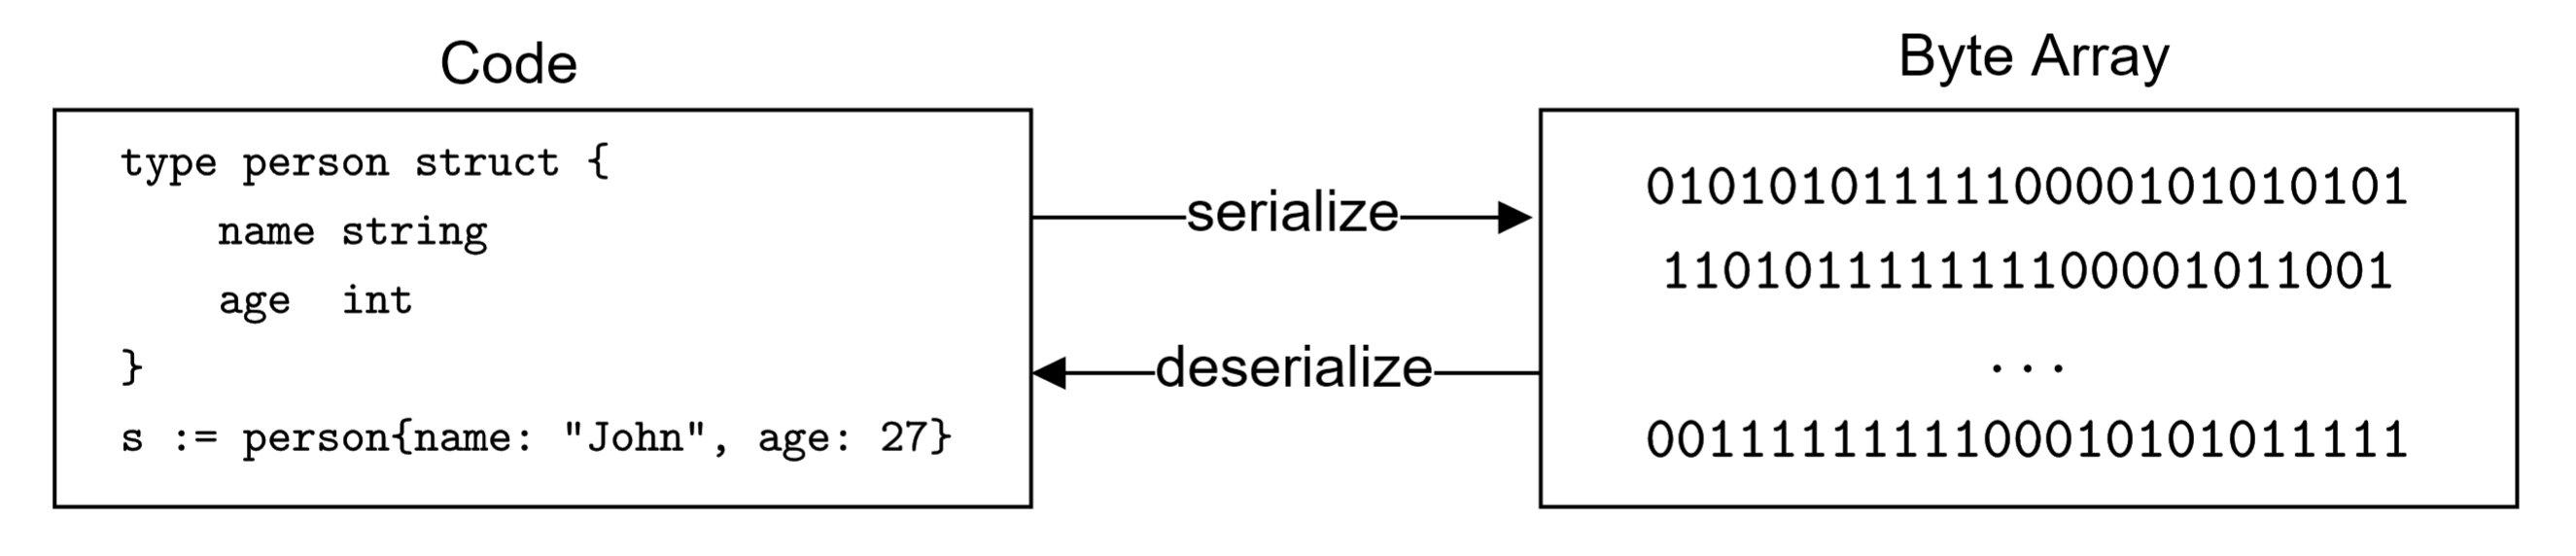
\includegraphics[width=1\textwidth]{Sections/rpc/ser.png}
    \caption{Serialization and Deserialization of data.}
    \label{fig:ser_deser}
\end{figure}

\noindent
There is one cardinal rule to remember when dealing with RPCs:
\begin{theo}[Network Reliability]

    \begin{center}
        \Large{\textbf{The network is always unreliable.}}
    \end{center}

    \vspace{1em}

    \noindent
    That is to say, the network can drop packets, delay messages, or deliver them out of order. Anything that 
    can go wrong will go wrong.
\end{theo}

\noindent
To handle network unreliability, we'll first consider two failure models:

\begin{Def}[At-least-once \& At-most-once]

    \begin{itemize}
        \item \textbf{At-least-once:} Ensures that the RPC call is delivered to the server at least once, regardless of failures. Though additional methods like IDs to ensure duplicated calls are handled server-side.
        \item \textbf{At-most-once:} Ensures that the RPC call is delivered at most once. So even if the call fails, it won't be retried. So messages may be lost if the server fails to receive them.
    \end{itemize}
\end{Def}

\newpage

\noindent
For our communication to work \textit{reliably} we need At-least-once and At-most-once with unlimited tries coupled by 
a fault-tolerant implementation. This brings us to the \textbf{GO RGC library}.

\begin{Def}[Go RPC Library]

    The Go RPC library provides a simple way to implement RPCs in the programming language Go. This gives us:
    \begin{itemize}
        \item At-most-once model with respect to a single
        client-server
        \item Built on top of single \textbf{TCP connection} (Transport Layer Protocol). This protocol ensures reliable communication between client and server.
        \item Returns error if reply is not received, e.g.,
        connection broken (TCP timeout)
    \end{itemize}
\end{Def}

\noindent
Now to discuss briefly how a basic TCP connection is made:
\begin{Def}[Establishing a TCP Connection (SYN ACK)]

    First a three-way handshake is a method used in a TCP/IP network to create a connection between a local host/client and server. 
    It is a three-step method that requires both the client and server to exchange \textbf{SYN (synchronize)}
     and \textbf{ACK (acknowledgment)}.
     \begin{enumerate}
        \item The client sends a SYN packet to the server requesting to synchronize sequence numbers.
        \item The server responds with a SYN-ACK packet, acknowledging the request and sending its own SYN request.
        \item The client responds with an ACK packet, acknowledging the server's SYN request.
     \end{enumerate}
    
    \noindent
    After the three-way handshake, the connection is established and the client and server can communicate exchanging SYN and ACK data-packets.
    To end the connection another three-way handshake takes placed, where instead SYN, \textbf{FIN (finish)} is used.
\end{Def}

\noindent
Given this implementation, we approach somewhere in the realm of an \textbf{Exactly-Once model}:

\begin{Def}[Exactly-Once Model]

    The Exactly-Once model guarantees that a message is delivered exactly once to the recipient. Meaning, messages aren't duplicated, lost, or delivered out of order.
    However, In practice, data packets might do all of the above. Though with the right
    protocols in place, we can ensure order of logic is preserved.
\end{Def}

\newpage 
\noindent
Below we illustrate a simple TCP connection:
\begin{figure}[h]
    \centering
    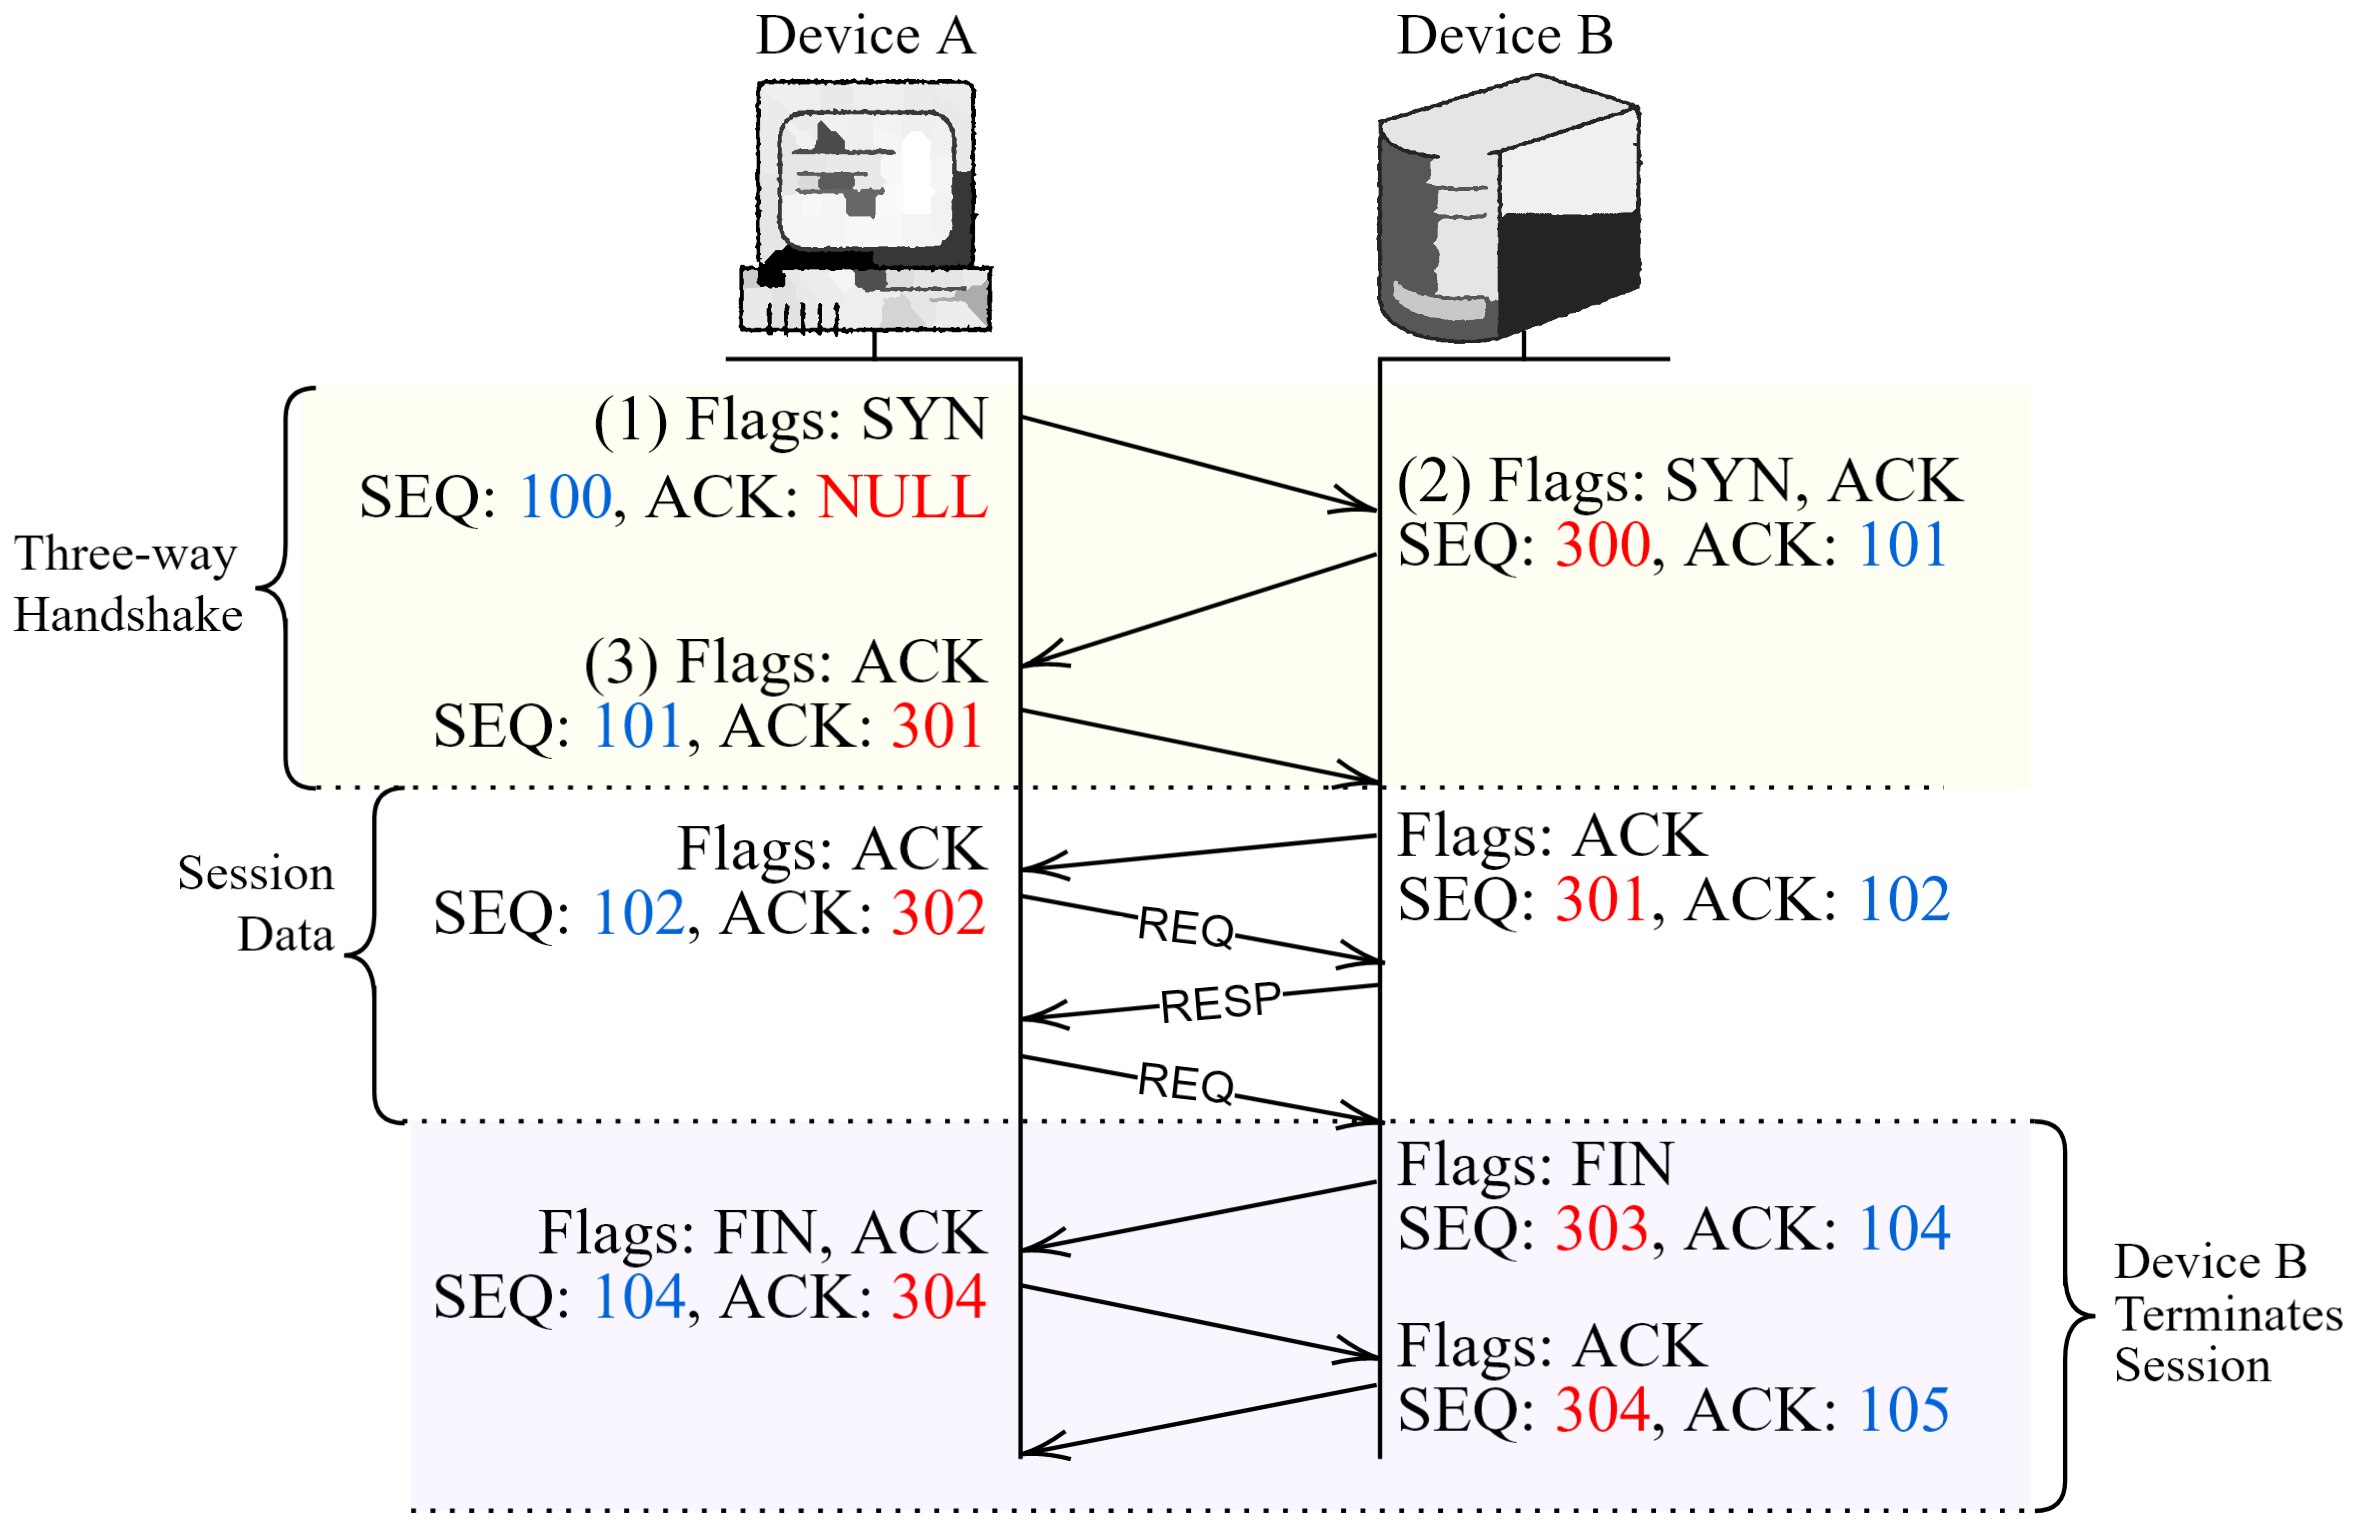
\includegraphics[width=1\textwidth]{Sections/rpc/sync.png}

    \vspace{1em}
    \caption{TCP Handshake, data transfer, and session termination.
    Here the client (Device A) begins a three-way handshake with the server (Device B) to establish a connection. Both start with 
    arbitrary sequence numbers for security purposes. With each packet received the two devices increment their sequence numbers accordingly.\\
    }
    \label{fig:tcp}
\end{figure}

\vspace{-1em}
\begin{Tip} If there still resides curiosity for the networking aspect of RPCs, consider reading our other notes:
    \href{https://github.com/Concise-Works/Cyber-Security/blob/main/main.pdf}{https://github.com/Concise-Works/Cyber-Security/blob/main/main.pdf}
\end{Tip}

\subsection{Asynchronous Function Calls}
Let's begin to discuss how functions can run simultaneously using Go's \textbf{goroutines}:
\begin{Def}[Asynchronous Function Calls]

    An \textbf{asynchronous function call} is a function that executes independently of the main program flow, enabling tasks to run concurrently or in parallel.

\end{Def}
\newpage

\noindent
To illustrate the difference between synchronous and asynchronous function calls, consider the following diagram:

\begin{figure}[h]
    \centering
    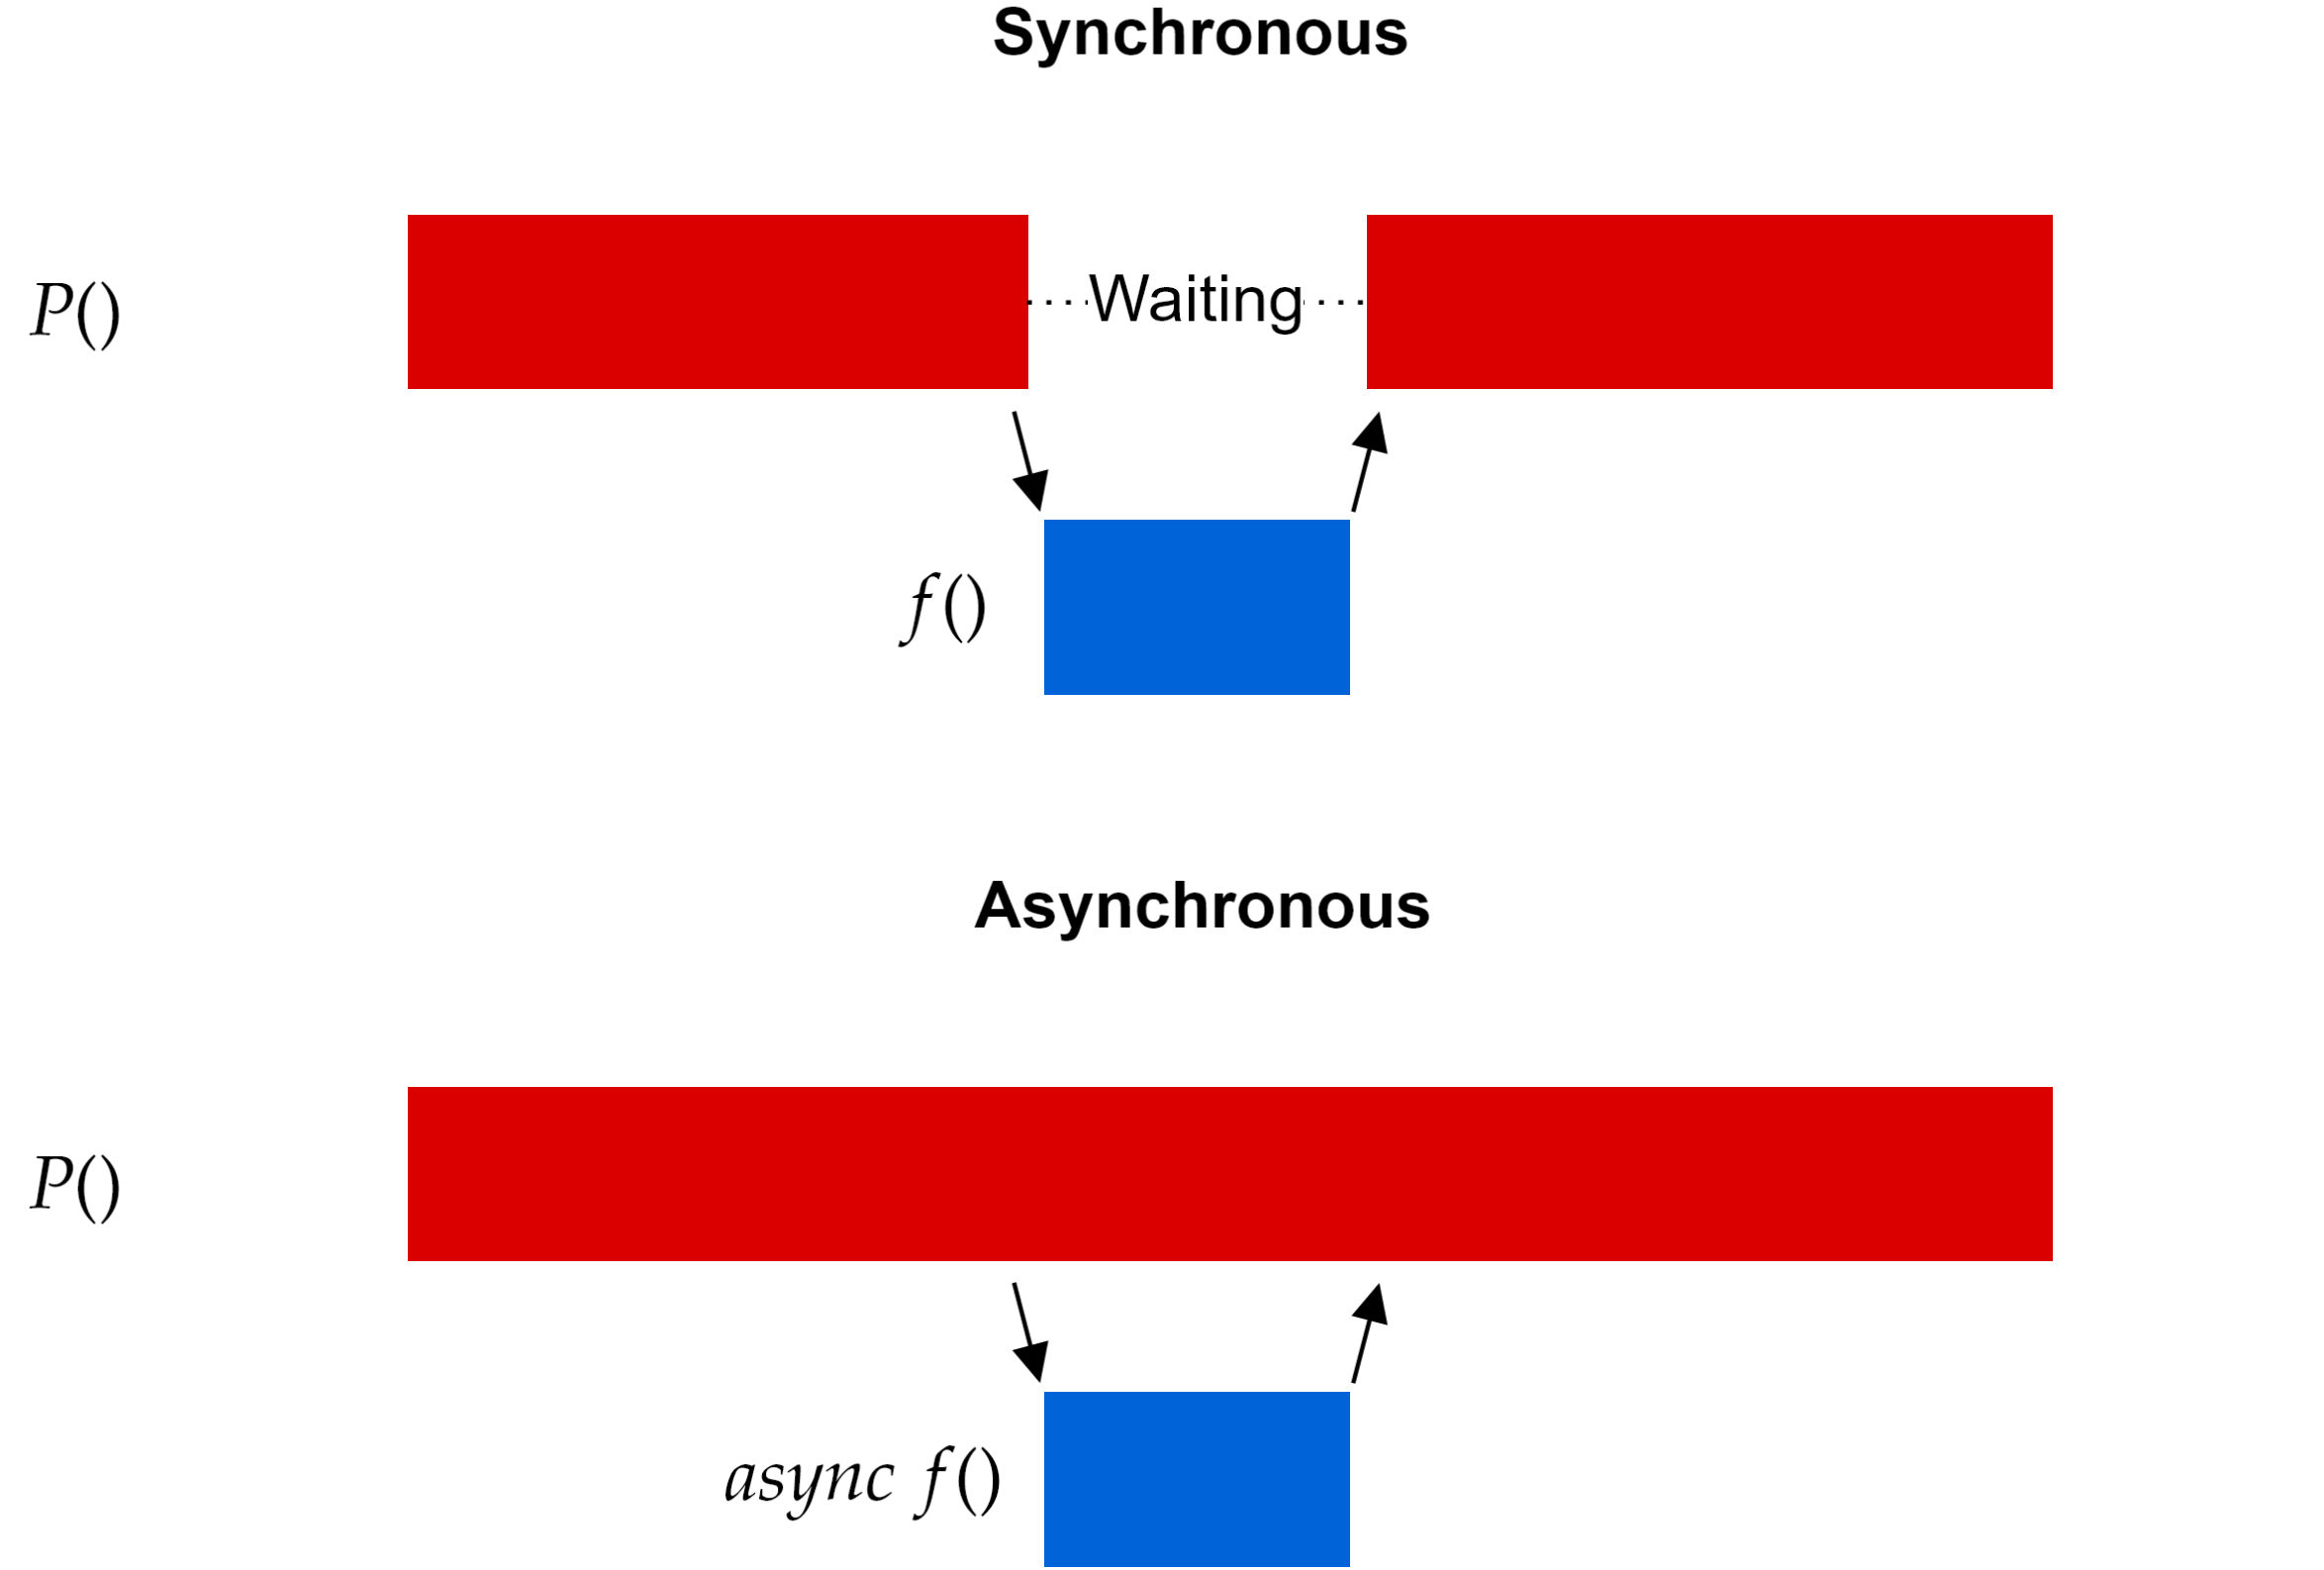
\includegraphics[width=1\textwidth]{Sections/rpc/Async.png}
    \caption{Synchronous vs. Asynchronous Function Calls.}
    \label{fig:sync_async}
\end{figure}

\noindent
\begin{itemize}
\item Function $P()$ (above) is the main function for which our program is running. It makes a synchronous call to function $f()$, which blocks the main program flow until $f()$ completes.
\item In contrast, function $P()$ (below) instead makes an asynchronous call to function $f()$, allowing the main program to continue executing while $f()$ runs independently.
\end{itemize}

\noindent
\begin{Def}[Asynchronous Function Calls in Go: Goroutines]

    A \textbf{goroutine} is a \textbf{lightweight} (lower memory overhead and scheduling cost compared to traditional OS threads)
    concurrent execution thread in Go. Goroutines enable functions to run asynchronously. Unlike traditional operating system threads, goroutines are managed by Go's runtime.
    
    A goroutine is created using the \snippet{go} keyword before a function call, signaling to the Go runtime to run the function asynchronously from the main program flow.
    
\end{Def}

\newpage 

\noindent
The below details the Go runtime scheduler. \textbf{Note}: that overtime the Go runtime's algorithm may change to improve 
performance. This isn't key to understanding the content of this text, but is provided for completeness sake. Here---at the time of writing---is how it works at a high-level:

\vspace{2em}
\begin{Def}[Go Runtime Scheduler]

    The Go runtime scheduler is responsible for managing goroutines via three conceptual entities:
\textbf{The Go Scheduler: G, M, P}
\begin{itemize}
    \item \textbf{G (Goroutine):} A goroutine that holds the code to be executed.
    \item \textbf{M (Thread):} An OS thread that executes Go code via system calls or remains idle.
    \item \textbf{P (Processor):} Represents resources needed to execute code. The number of processors is determined by \snippet{GOMAXPROCS}.
\end{itemize}

\noindent
If there are multiple goroutines, threads, and available processors, the scheduler matches them as follows:
\begin{itemize}
    \item Many \textbf{Gs} (goroutines) are mapped to available \textbf{Ms} (OS threads), which execute them using \textbf{Ps} (processors) as execution resources.
\end{itemize}

\noindent
\textbf{Queues in the Scheduler}
\begin{itemize}
    \item \textbf{Global Run Queue (GRQ):} Holds all new goroutines that are yet to execute.
    \item \textbf{Local Run Queue (LRQ):} Holds goroutines that are assigned to a specific \textbf{P}.
\end{itemize}

\noindent
For example, let the processors in the scheduler be defined as 
$
P = \{ P_1, P_2, \dots, P_n \}
$
where \( n = \texttt{GOMAXPROCS} \). Then the scheduler follows the following steps:
\begin{enumerate}
    \item If \( P_1 \) has no more goroutines to execute, it follows these steps:
    \begin{enumerate}
        \item Check \textbf{GRQ} for a \textbf{G} (goroutine) roughly \textit{1/61th of the time}.
        \item If nothing is found, check \textbf{LRQ} again.
        \item If nothing is found, attempt to \textbf{steal} work from other \textbf{Ps}.
        \item If nothing is found, check \textbf{GRQ} one last time.
        \item Finally, \textbf{poll the network} (i.e., check for incoming network work).
    \end{enumerate}
\end{enumerate}
\end{Def}

\vfill
\begin{center}
    
    \textit{The next page includes a diagram of the Go runtime scheduler above.}
\end{center}

\vfill
\newpage
\noindent
To illustrate the Go runtime scheduler on a high-level, consider the following diagram in contrast to Figure \ref{fig:kernel}: 

\begin{figure}[h]
    
    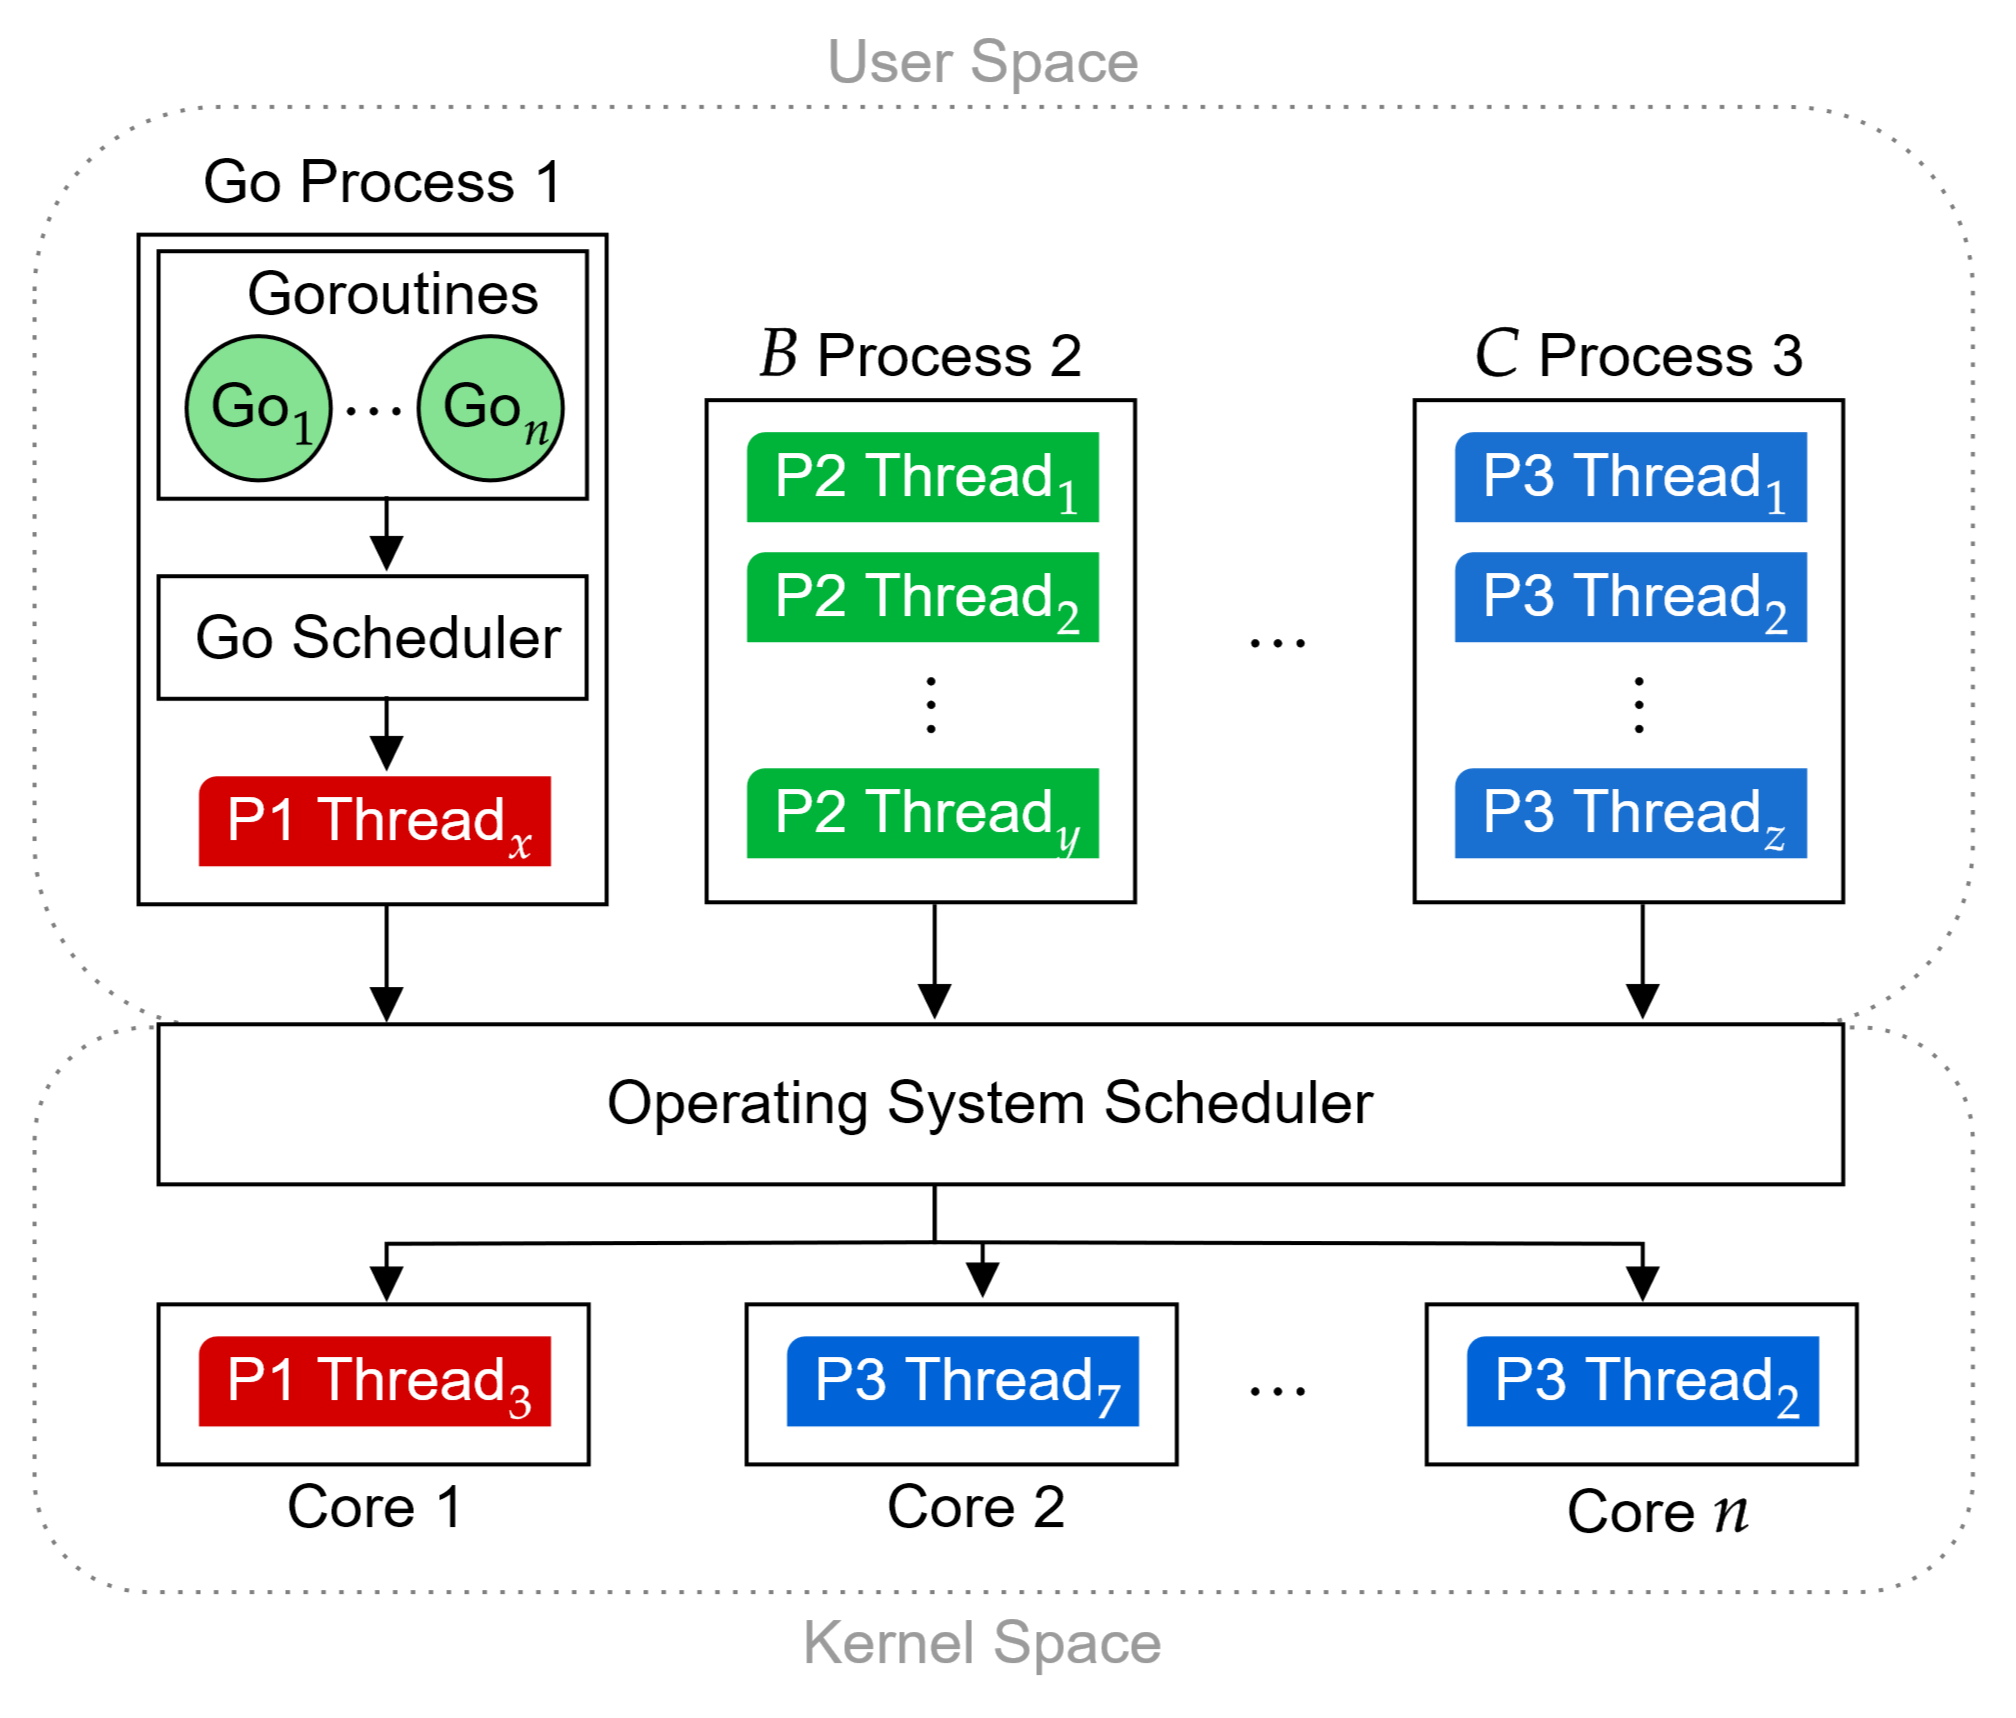
\includegraphics[width=1\textwidth]{Sections/rpc/high_sched.png}
    \caption{Go runtime scheduler with G, M, P entities.}
    \label{fig:go_scheduler}
\end{figure}
\noindent
Where the system has many different processes $B$, $C$ and so on, we focus on the process that contains an instance of the Go runtime scheduler.
Within this process each goroutine is scheduled by the Go runtime scheduler. The Go scheduler determines the number of threads needed
and assigns goroutines to them. The process then presents these threads to the OS Scheduler which assigns them to the available cores.

In particular, \textbf{The OS has the final decision on which threads run on which cores.} The Go runtime scheduler only manages what threads to present.
This is still helpful as the Go runtime can context switch the threads between goroutines before the handoff. Hence, the name \textbf{lightweight threads}, as 
context switching for the OS is expensive.

\newpage 
\noindent
In particular we zoom in on the Go runtime scheduler of a single process: 
\begin{figure}[h]
    
    \hspace{-3em}
    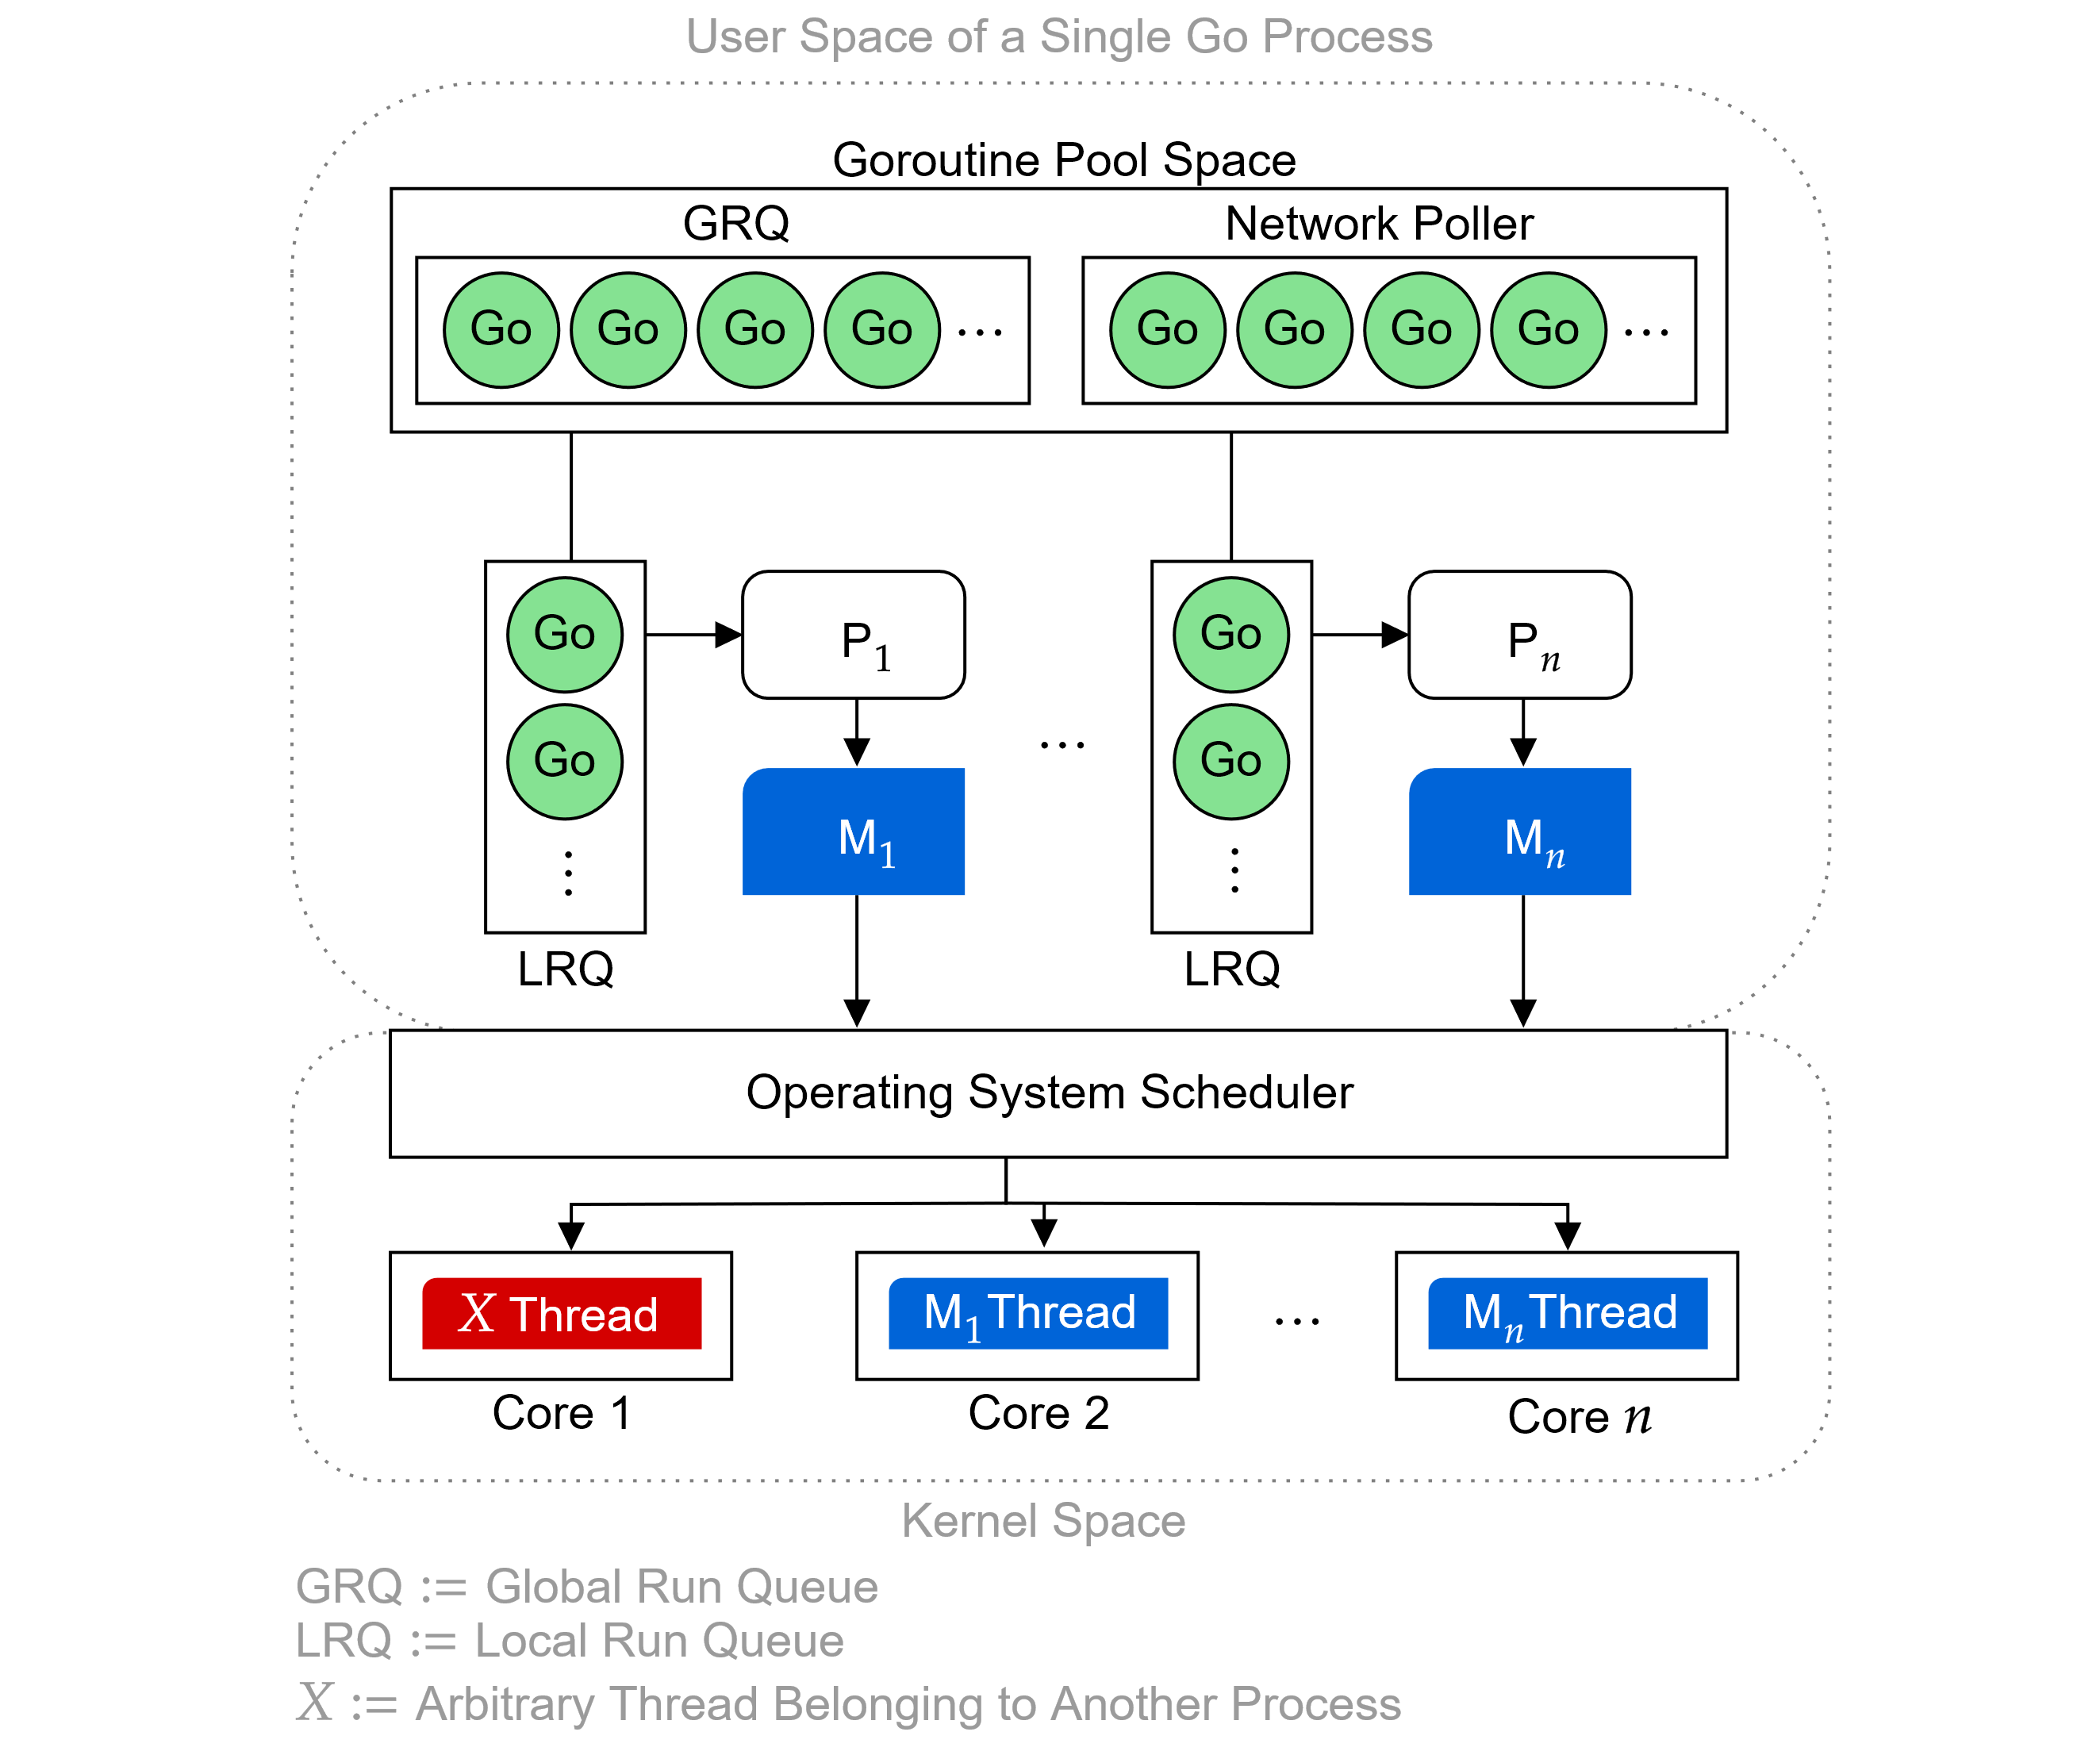
\includegraphics[width=1.1\textwidth]{Sections/rpc/sheduler.png}
    \caption{Go runtime scheduler within a single process.}
    \label{fig:scheduler}
\end{figure}

\noindent
Here our ``Goroutine Pool Space'' represents the latent goroutines waiting to be executed. 
We populate the LRQs of each P and their assigned M thread. The Ms are presented to the OS Scheduler. Moreover, 
the $X$ is some arbitrary thread belonging to another process on the system.\\
For emphasis
\begin{theo}[Go Runtime Scheduler vs. OS Scheduler]

    The Go runtime only manages threads to present; The OS schedules threads to cores.
\end{theo}
\newpage 

\noindent
In all, the asynchronous nature of goroutines may create undefined behavior if not handled properly.
\begin{Example}[Count to n using Goroutines]

    \label{ex:goroutine}
    Consider the following Go program that counts to $n$ using a goroutine:
    \begin{lstlisting}[language=Go, caption=Goroutine Example: Count to n, label={lst:goroutine}, numbers=none]
    package main // Required for Go programs to run as executables
    import (
        "fmt"
        "time"
    ) // Import required packages : fmt for printing and time for sleep
    
    // ''i:=1'' is short for ''var i int = 0''
    func countUp(n int) {
        for i := 1; i <= n; i++ {
            // Anonymous function declared as a goroutine
            go func() {
                fmt.Println("Goroutine:", i)
            }()
        }
    }
    // Main entry point of the program
    func main() {
        countUp(5)
    }
    \end{lstlisting}
    \noindent
    However, this won't print anything as the main function exits before the independent goroutine can finish. A simple fix we'll do for now is put a sleep to wait for the goroutine to finish.
    \begin{lstlisting}[language=Go, caption=Adding a Sleep to Wait for Goroutine, label={lst:sleep}, numbers=none]
        func main() {
            countUp(5) // contains a goroutine
            time.Sleep(2 * time.Second) // Wait for goroutine to finish
            fmt.Println("Main function exits")
        }
    \end{lstlisting}

    Ensuring the main function waits for the goroutine to finish.
\end{Example}

\begin{theo}[Main Goroutine Thread]

    the main function of a goroutine is too a kind of goroutine. We may refer to it as the \textbf{main goroutine} or \textbf{main thread}.
    In particular, the main goroutine is the first to run and may finish before any other goroutine.
\end{theo}


\newpage 

\noindent
Though since calls happen independent of each other means they happen simultaneously.
\begin{Example}[Count to n using Goroutines Corollary]

    \label{ex:goroutine_corollary}
    Continuing off from the previous example (\ref{ex:goroutine}), we'll get an output such as:
    \begin{lstlisting}[language=Go, caption=Output of Goroutine Example, label={lst:output}, numbers=none]
    ...
    func countUp(n int) {
        for i := 1; i <= n; i++ {
            go func() {
                fmt.Println("Goroutine:", i)
            }()
        }
    }

    func main() {
        countUp(5) // Runs countUp concurrently
        time.Sleep(2 * time.Second) // Wait for goroutine to finish
        fmt.Println("Main function exits")
    }

    /* Output:
    Goroutine: 4
    Goroutine: 3
    Goroutine: 5
    Goroutine: 2
    Goroutine: 1
    Main function exits
    */
    \end{lstlisting}
    \noindent
    The goroutine spawns multiple threads for each print of counter $i$. Therefore the order at which they execute is 
    up to the Go runtime scheduler.
\end{Example}

\begin{theo}[Goroutines and Multithreading]

    Goroutines will attempt to run on multiple threads to achieve parallelism. However, if there isn't enough cores available, 
    threads will run concurrently on the same core.

    To declare how many cores can use, \snippet{runtime.GOMAXPROCS} from the \snippet{runtime} package can be used.
    \begin{lstlisting}[language=Go, caption=Setting the Number of Cores for Goroutines, label={lst:cores}]
        import "runtime"
        runtime.GOMAXPROCS(n) // n = number of cores to use
    \end{lstlisting}
    \noindent
    By default, Go will use the number of cores available on the machine.
\end{theo}

\newpage 

\noindent
Try these examples out in Go to get a feel for how goroutines work.

\begin{Def}[Installing and Running Go Programs]

    First, install Go from the official website: \href{https://go.dev/doc/install}{https://go.dev/doc/install}.
    The Go file extension is \snippet{.go}:
    \begin{itemize}
        \item \textbf{To run a Go program:} Use the command \snippet{go run <filename>.go}.
        \item \textbf{To build a Go program:} Use the command \snippet{go build <filename>.go} to create an executable.
        Then run the program in a terminal via \snippet{./<filename>}.
    \end{itemize}
\end{Def}

\begin{Tip}
    This text will teach the necessary components as we go along. However, if one wishes to learn on their own 
    a little first, consider the following resource: \href{https://gobyexample.com/}{https://gobyexample.com/}.
    Though this text does assume prior programming knowledge and should be follow-able without the resource.
\end{Tip}
\subsection{Synchronization: Data Races \& Deadlocks}
\noindent
Asynchronous functions introduces a problem: If two threads access the same memory location at the same time,
we face corruption of data as they try to write over each other:
\begin{Def}[Data Race]

    A \textbf{data race} occurs when multiple threads or goroutines access the same memory location concurrently, and at least one of the accesses is a write operation, without proper synchronization. This leads to undefined behavior, including inconsistent data and unpredictable program execution.
    \end{Def}
        
\noindent
To avoid data races we implement the following strategy:
\begin{Def}[Mutex (Mutual Exclusion)]

    A \textbf{mutex} (short for \emph{mutual exclusion}) is a synchronization primitive that prevents multiple threads from simultaneously accessing shared resources. This allows a single thread to place a \textbf{lock} on the resource, ensuring exclusive access until the lock is released.
\end{Def}

\newpage
    
\noindent
Go has their own mutex implementation:
\begin{Def}[Go Mutex]
    
    In Go, the \snippet{sync.Mutex} type provides a way to control access to shared data. A \texttt{Mutex} has two main methods:
    \begin{itemize}
        \item \snippet{Lock()}: declares that the current goroutine from which it resides has exclusive access to the resource.
        \item \snippet{Unlock()}: Releases the mutex, allowing other goroutines to access the resource.
    \end{itemize}
\end{Def}
    
\vspace{-.5em}
\begin{Example}[Increasing a Counter Variable with Goroutines]

    \label{ex:counter}
    Consider the following example where a function \snippet{incCounter()} increments a shared counter variable:
    \begin{lstlisting}[language=Go, caption=Incrementing a Counter Variable, label={lst:counter}, numbers=none]
    ...
    var counter int // declaring global counter variable
    
    func incCounter() {
        counter = counter + 1
    }

    func main() {
        // forloop spawning an instance of incCounter() in a goroutine
        for i := 0; i < 1000; i++ {
            go func() {
                incCounter()
            }()
        }
        time.Sleep(5 * time.Second)
        fmt.Println("Counter:", counter)
    }
    /* Output: Counter: 982 */
    \end{lstlisting}
    \noindent
    By the end of the forloop, the counter will most often not be 1000. This is due to counter having 
    a different state in each goroutine. To fix this, we'll use a mutex. So it is very possible that the first 2 goroutines 
    look like this:
    \begin{itemize}
        \item Goroutine 1: \snippet{counter = 0 + 1}
        \item Goroutine 2: \snippet{counter = 0 + 1}
    \end{itemize}
    \noindent
    Where all three goroutines see the counter as 0, increment it all setting it to 1.
\end{Example}

\newpage 

\noindent
Now to fix the previous example (\ref{ex:counter}) using a mutex:

\begin{Def}[Increasing a Counter Variable with a Mutex]

    To ensure a global variable counter is incremented correctly, we'll use a mutex:
    \begin{lstlisting}[language=Go, caption=Using a Mutex to Increment a Counter Variable, label={lst:mutex}, numbers=none]
    ... // imported the "sync" package for the mutex
    var counter int
    var mu sync.Mutex // declaring a mutex

    func incCounter() {
        mu.Lock() // Lock the mutex
        counter = counter + 1
        mu.Unlock() // Unlock the mutex
    }

    func main() {
        for i := 0; i < 1000; i++ {
            go func() {
                incCounter()
            }()
        }
        time.Sleep(5 * time.Second)
        fmt.Println("Counter:", counter)
    }

    /* Output:
    Counter: 1000
    */
    \end{lstlisting}

    \noindent
    By using a mutex, we ensure that only one goroutine can access the shared counter variable at a time.
    \underline{\textbf{Important Note:} This does not ensure the order in which the goroutines run.}
\end{Def}

\noindent
Though with mutexes may come another problem, what if a goroutine never releases the lock?
\begin{Def}[Deadlock]

    A \textbf{deadlock} occurs when two or more asynchronous processes are waiting for each other to release a resource, preventing all processes from progressing. This results in a program that hangs indefinitely.
\end{Def}
\noindent
In a large project a logical mistake in a sea of processes can lead to a deadlock. 

\newpage

\noindent
\begin{Example}[Deadlock Scenario]
    
    Say we have functions \snippet{task1()} and \snippet{task2()} that each require a mutex lock:
    \begin{lstlisting}[language=Go, caption=Deadlock Scenario, label={lst:deadlock}, numbers=none]
    ... // dots represent some passage of code

    go func task1() {
        lockA.lock() ... lockB.lock()
        ...
        lockB.unlock() ... lockA.unlock()
    }

    go func task2() {
        lockB.lock() ... lockA.lock()
        ...
        lockA.unlock() ... lockB.unlock()
    }
    
    ...
    \end{lstlisting}
    Depending on how the scheduler runs, these two tasks will lock each other out, halting the program indefinitely.
\end{Example}


\subsection{References \& Pointers in Go}

\noindent
In Go, problems may arise from how Go deals with scoped variables:
\begin{Def}[Reference vs. Value Types]

    In Go, variables can be either \textbf{reference types} or \textbf{value types}:
    \begin{itemize}
        \item \textbf{Reference Types:} Point to a memory location where the actual data is stored. Changes to the reference type will affect all variables pointing to the same memory location.
        \item \textbf{Value Types:} Store the actual data in memory. Changes to a value type will not affect other variables.
    \end{itemize}
\end{Def}

\begin{Def}[Closures and Reference Types]

    In Go, if a variable isn't explicitly pass to a function, but is rather accessible from the function's scope, it is considered a \textbf{closure}. This 
    closure is a reference to the variable, not the data itself.
\end{Def}

\newpage 

\begin{Example}[Closures and Goroutines]

    Let \snippet{data} be some channel and \snippet{do\_something()} be some function that returns a value:

    \begin{lstlisting}[language=Go, numbers= none]
    ...
    batch := 0
    for i := 0; i < k; i++ {
        go func() {
            data <- do_something(batch)
        }()
    }
    batch++
    ...
    \end{lstlisting}

    \noindent
    Here, the \snippet{go func} closure will reference the \snippet{batch} variable, not the value. Hence the main program flow (the main thread) might increment \snippet{batch} 
    before the goroutine runs, leading to undefined behavior. To fix this, we pass the variable as an argument to the goroutine:

    \begin{lstlisting}[language=Go, numbers= none]
    ...
    batch := 0
    for i := 0; i < k; i++ {
        go func(batch int) {
            data <- do_something(batch)
        }(batch)
    }
    batch++
    ...
    \end{lstlisting}

    \noindent
    Now the goroutine will receive the value of \snippet{batch} at the time of the loop iteration.
\end{Example}
    
\noindent
Many data-structures in Go pass by value. Pointers ensure we are updating the original object:
\begin{Def}[Passing Pointers in Go]

    Pointers in Go pass the memory address of a variable via the \snippet{\&} operator. To access the value stored at the memory address, use the \snippet{*} operator. E.g.,
    \begin{lstlisting}[language=Go, numbers=none]
    var x int = 5
    var y *int = &x // y stores the memory address of x
    fmt.Println(*y) // Prints the value stored at the memory address
    \end{lstlisting}
\end{Def}

\newpage 

\subsection{Waiting for Goroutines to Finish}
\noindent
Previously we used \snippet{time.Sleep()} to wait for goroutines to finish; However, Go provides a solution to this problem:

\begin{Def}[Wait Groups]

    A \textbf{wait group} is a synchronization primitive in Go that allows the main program to wait for a collection of goroutines. 
    A wait group is a counter spawned with \snippet{sync.WaitGroup} and has three main methods:
    \begin{itemize}
        \item \snippet{Add(n int)}: Increments the wait group counter by \snippet{n}.
        \item \snippet{Done()}: Decrements the wait group counter by 1.
        \item \snippet{Wait()}: Blocks the main program until the wait group counter reaches 0.
    \end{itemize}
\end{Def}

\begin{Example}[Using Wait Groups]

    \label{ex:waitgroup}
    Let's consider the following example where we use a wait group to wait for goroutines to finish:
    \begin{lstlisting}[language=Go, numbers=none]
    ...
    var wg sync.WaitGroup // declaring a wait group
    var mu sync.Mutex 
    for i := 0; i < 1000; i++ {
        wg.Add(1) // Increment the wait group counter
        go func() {
            mu.Lock()
            incCounter()
            mu.Unlock()
            wg.Done() // Decrement the wait group counter
        }()
    }
    wg.Wait() // Wait for wg counter to reach 0
    \end{lstlisting}
    \noindent
\end{Example}

\noindent
An aside on a handy feature of Go: 
\begin{Def}[Deferred Function Calls]

    In Go, the \snippet{defer} keyword  \textbf{defers a function call} to run at the end of the innermost scoped function. 
    Deferred functions are often used to ensure cleanup tasks are executed, such as closing files or releasing resources.
\end{Def}

\begin{Example}[Deferred Function Calls]

    \label{ex:defer}
    Consider the previous example (\ref{ex:waitgroup}) with a deferred function call of \snippet{wg.Done()}:

    \begin{lstlisting}[language=Go, label={lst:defer}, numbers=none]
    ...
    for i := 0; i < 1000; i++ {
        wg.Add(1) 
        go func() {
            defer wg.Done() // Deferred function call
            mu.Lock() 
            incCounter()
            mu.Unlock() 
        }()
    }...
\end{lstlisting}
\noindent
The \snippet{wg.Done()} is deferred until the goroutine completes.
\end{Example}

\subsection{Sending Messages Between Goroutines}
\noindent
Now, say there are tasks $A$ and $B$, for which $B$ depends on the completion of $A$. Since $A$ and $B$ both run independently, we need a way for $B$ to wait for a signal from $A$. This is where \textbf{channels} come in:
\begin{Def}[Channels]

    A \textbf{channel} is a typed conduit through which goroutines communicate. Channels allow goroutines to send and receive data.
    Channels are created using the \snippet{make()} function with the \snippet{chan} keyword. Channels must be closed after use to prevent memory leaks with \snippet{close()}.
\end{Def}

\begin{figure}[h]
    \centering
    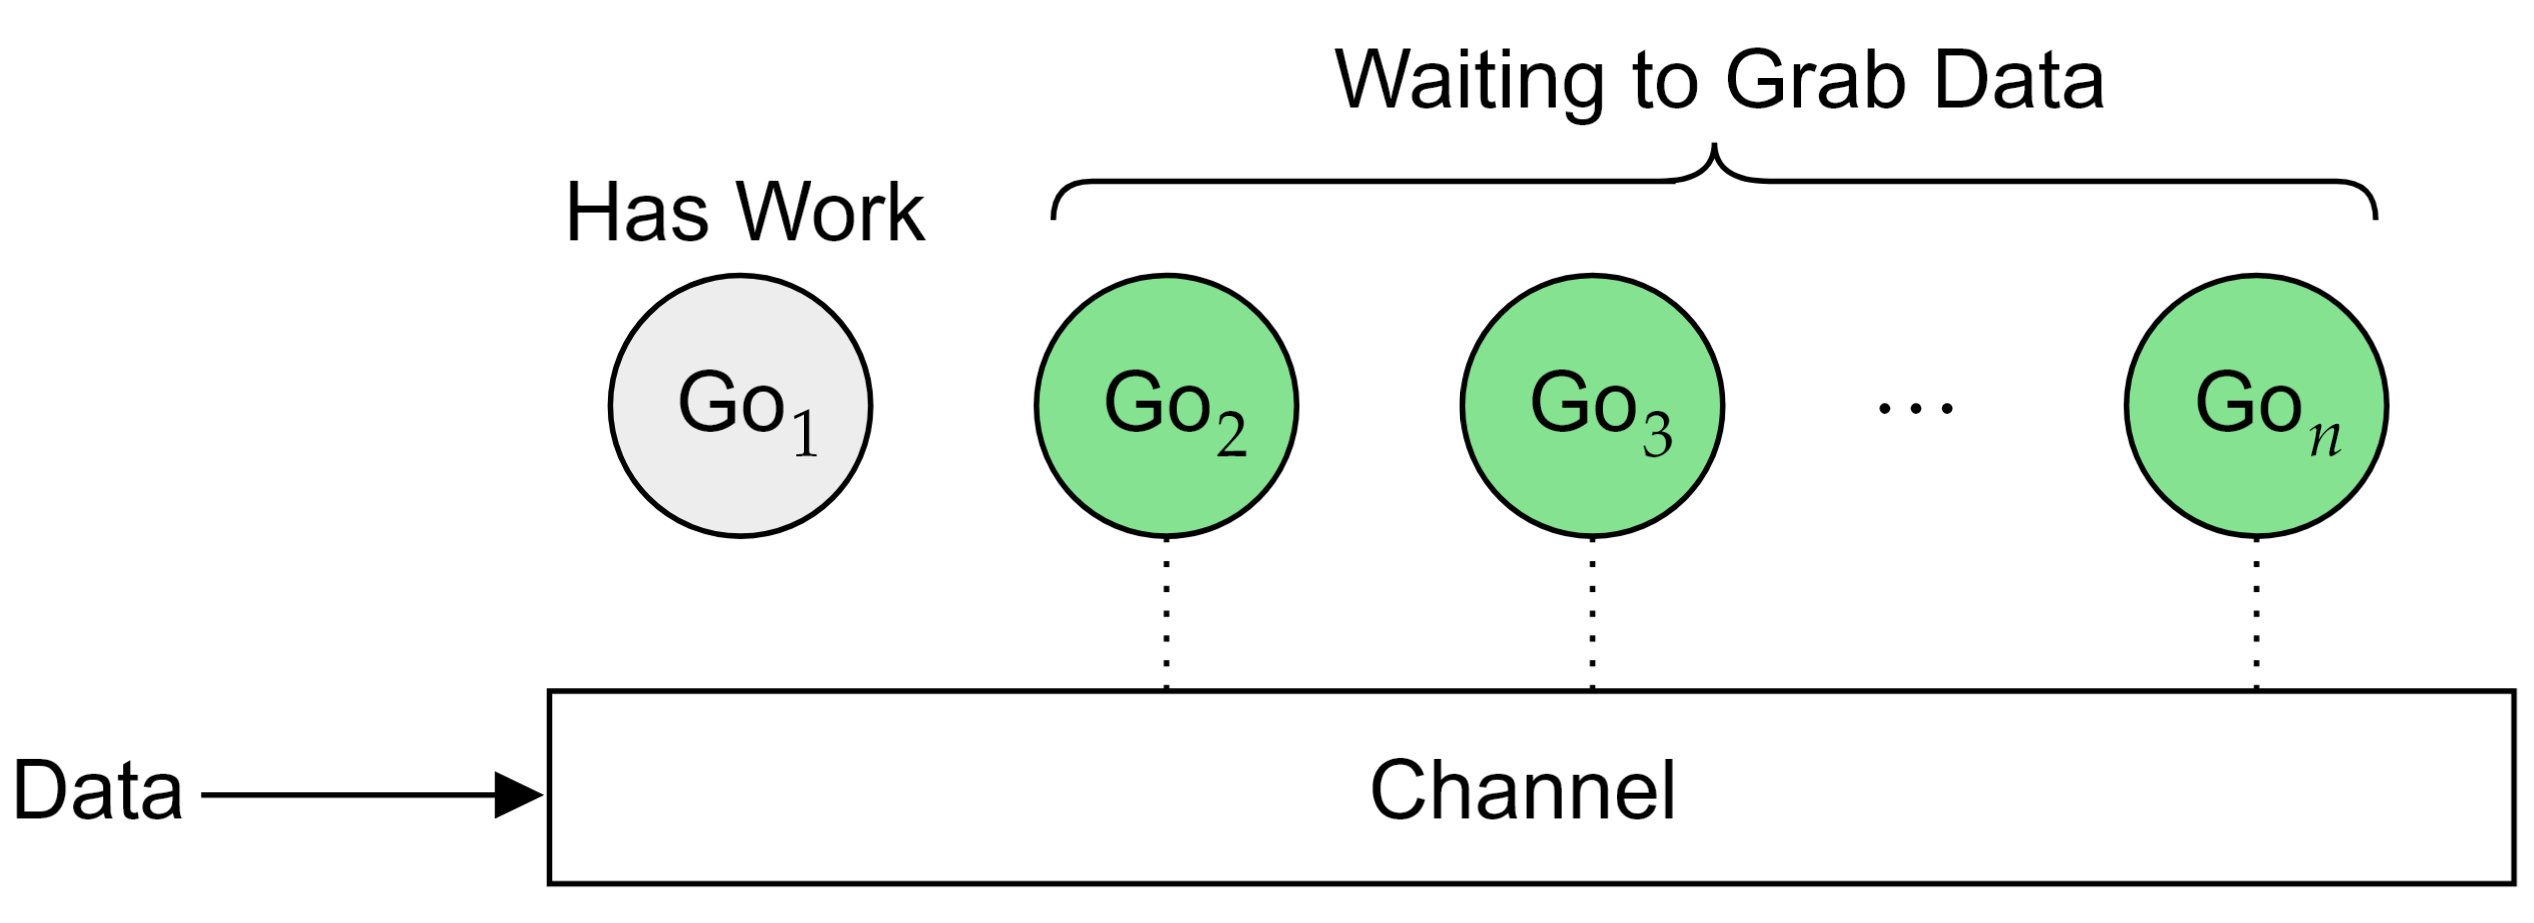
\includegraphics[width=0.8\textwidth]{Sections/rpc/channel.png}
    \caption{A collection of Goroutines competing for the next channel resource.}
    \label{fig:channel}
\end{figure}
\noindent
Note, despite the diagrams order of goroutines, the order in which they run is up to the Go runtime scheduler.

\begin{Example}[Synchronizing Incoming Data Processing with Channels]

    \label{ex:channels}
Consider the following example of downloading and processing data concurrently:
\begin{lstlisting}[language=Go, caption=Using Channels to Synchronize Downloading and Processing, label={lst:channels}, numbers=none]
    package main
    import (
        "fmt"
        "sync"
        "time"
    )

    // Download function simulates downloading data and sends a signal when done
    func download(i int, ch chan int) {
        fmt.Printf("Downloading: Resource_%d...\n", i)
        time.Sleep(5 * time.Second) // Simulating download time
        fmt.Printf("Download complete: Resource_%d\n", i)
        ch <- i // Send signal that download is complete
    }

    // Process function waits for a signal before processing
    func process(ch chan int, wg *sync.WaitGroup) {
        defer wg.Done()
        i := <-ch // Wait for download to complete
        fmt.Printf("Processing: Resource_%d...\n", i)
        time.Sleep(1 * time.Second) // Simulating processing time
        fmt.Printf("Processing complete: Resource_%d\n", i)
    }

    func main() {
        n := 5
        ch := make(chan int) // Unbuffered channel
        var wg sync.WaitGroup
        wg.Add(n)
        // Spawn n goroutines to download and process resources concurrently
        for i := 0; i < n; i++ {
            go download(i, ch)
            go process(ch, &wg)
        }

        wg.Wait()
        close(ch) // Close channel after all downloads are completed
        fmt.Println("Main function exits")
    }

    \end{lstlisting}
\end{Example}

\newpage 

\begin{theo}[Channel Types]

    In Go, channels can be either \textbf{unbuffered} or \textbf{buffered}:
    \begin{itemize}
        \item \textbf{Unbuffered Channels:} Require a sender and receiver to be ready to communicate. If the receiver is not ready, the sender will block until the receiver is ready.
        \item \textbf{Buffered Channels:} Allow a sender to send data to a channel without the receiver being ready. The channel will store the data until the receiver is ready.
    \end{itemize}
\end{theo}

\noindent
Unbuffered channels undergo a \textbf{handshake} process:
\begin{figure}[h]
    \centering
    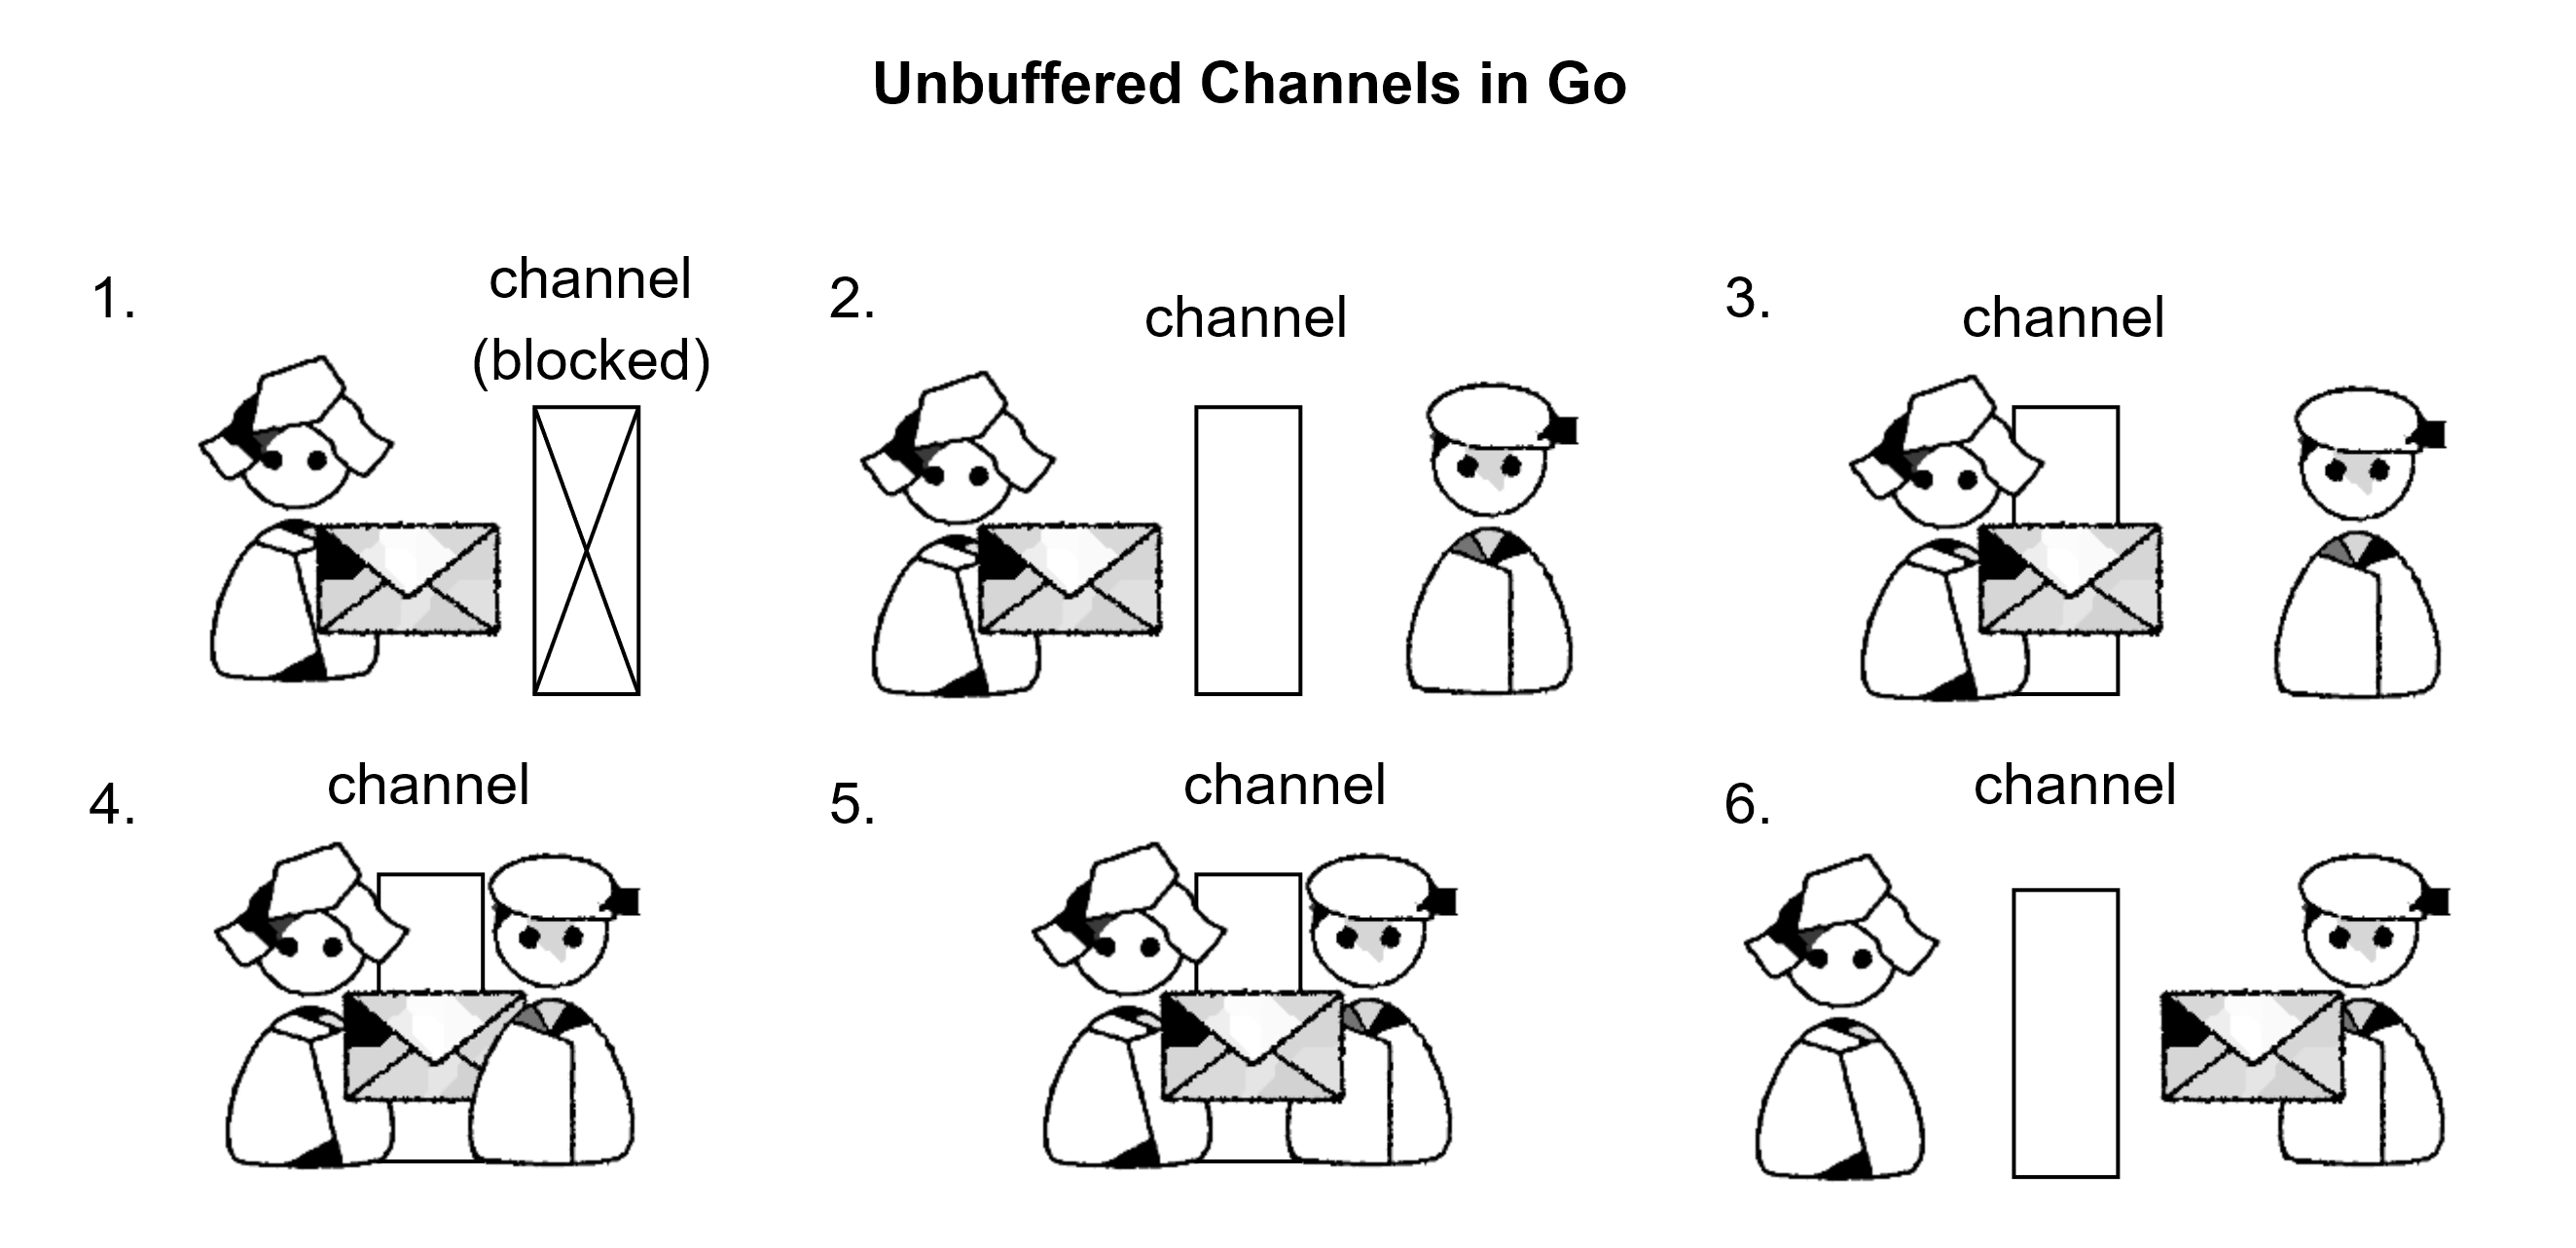
\includegraphics[width=1\textwidth]{Sections/rpc/unbuffered.png}
    \caption{Handshake process of an unbuffered channel.}
    \label{fig:handshake}
\end{figure}

\noindent
Say Alice (left) want to send a message to Bob (right) over a channel. (1) The channel is blocked until Bob is ready to receive. (2) The channel is no longer blocked 
read for the exchange. (3) Alice preforms a \textbf{send} and is locked into the operation until Bob \textbf{receives} the message. (4-5) Bob enters the channel and receives the message;
Both Alice and Bob are locked into the operation until the message exchange is complete.
(6) they both are free to continue their operations.\\

\begin{theo}[Unbeffered Blocking]
\noindent
Let $A$ and $B$ be two goroutines attempting to send messages over an unbuffered channel. 
If $A$ enters the channel first, $B$ will be blocked until $A$ finishes the transaction.
\end{theo}
The previous example (\ref{ex:channels}) uses an unbuffered channel.
\newpage 

\noindent
In contrast buffered channels allow for a more asynchronous approach:

\begin{figure}[h]
    \centering
    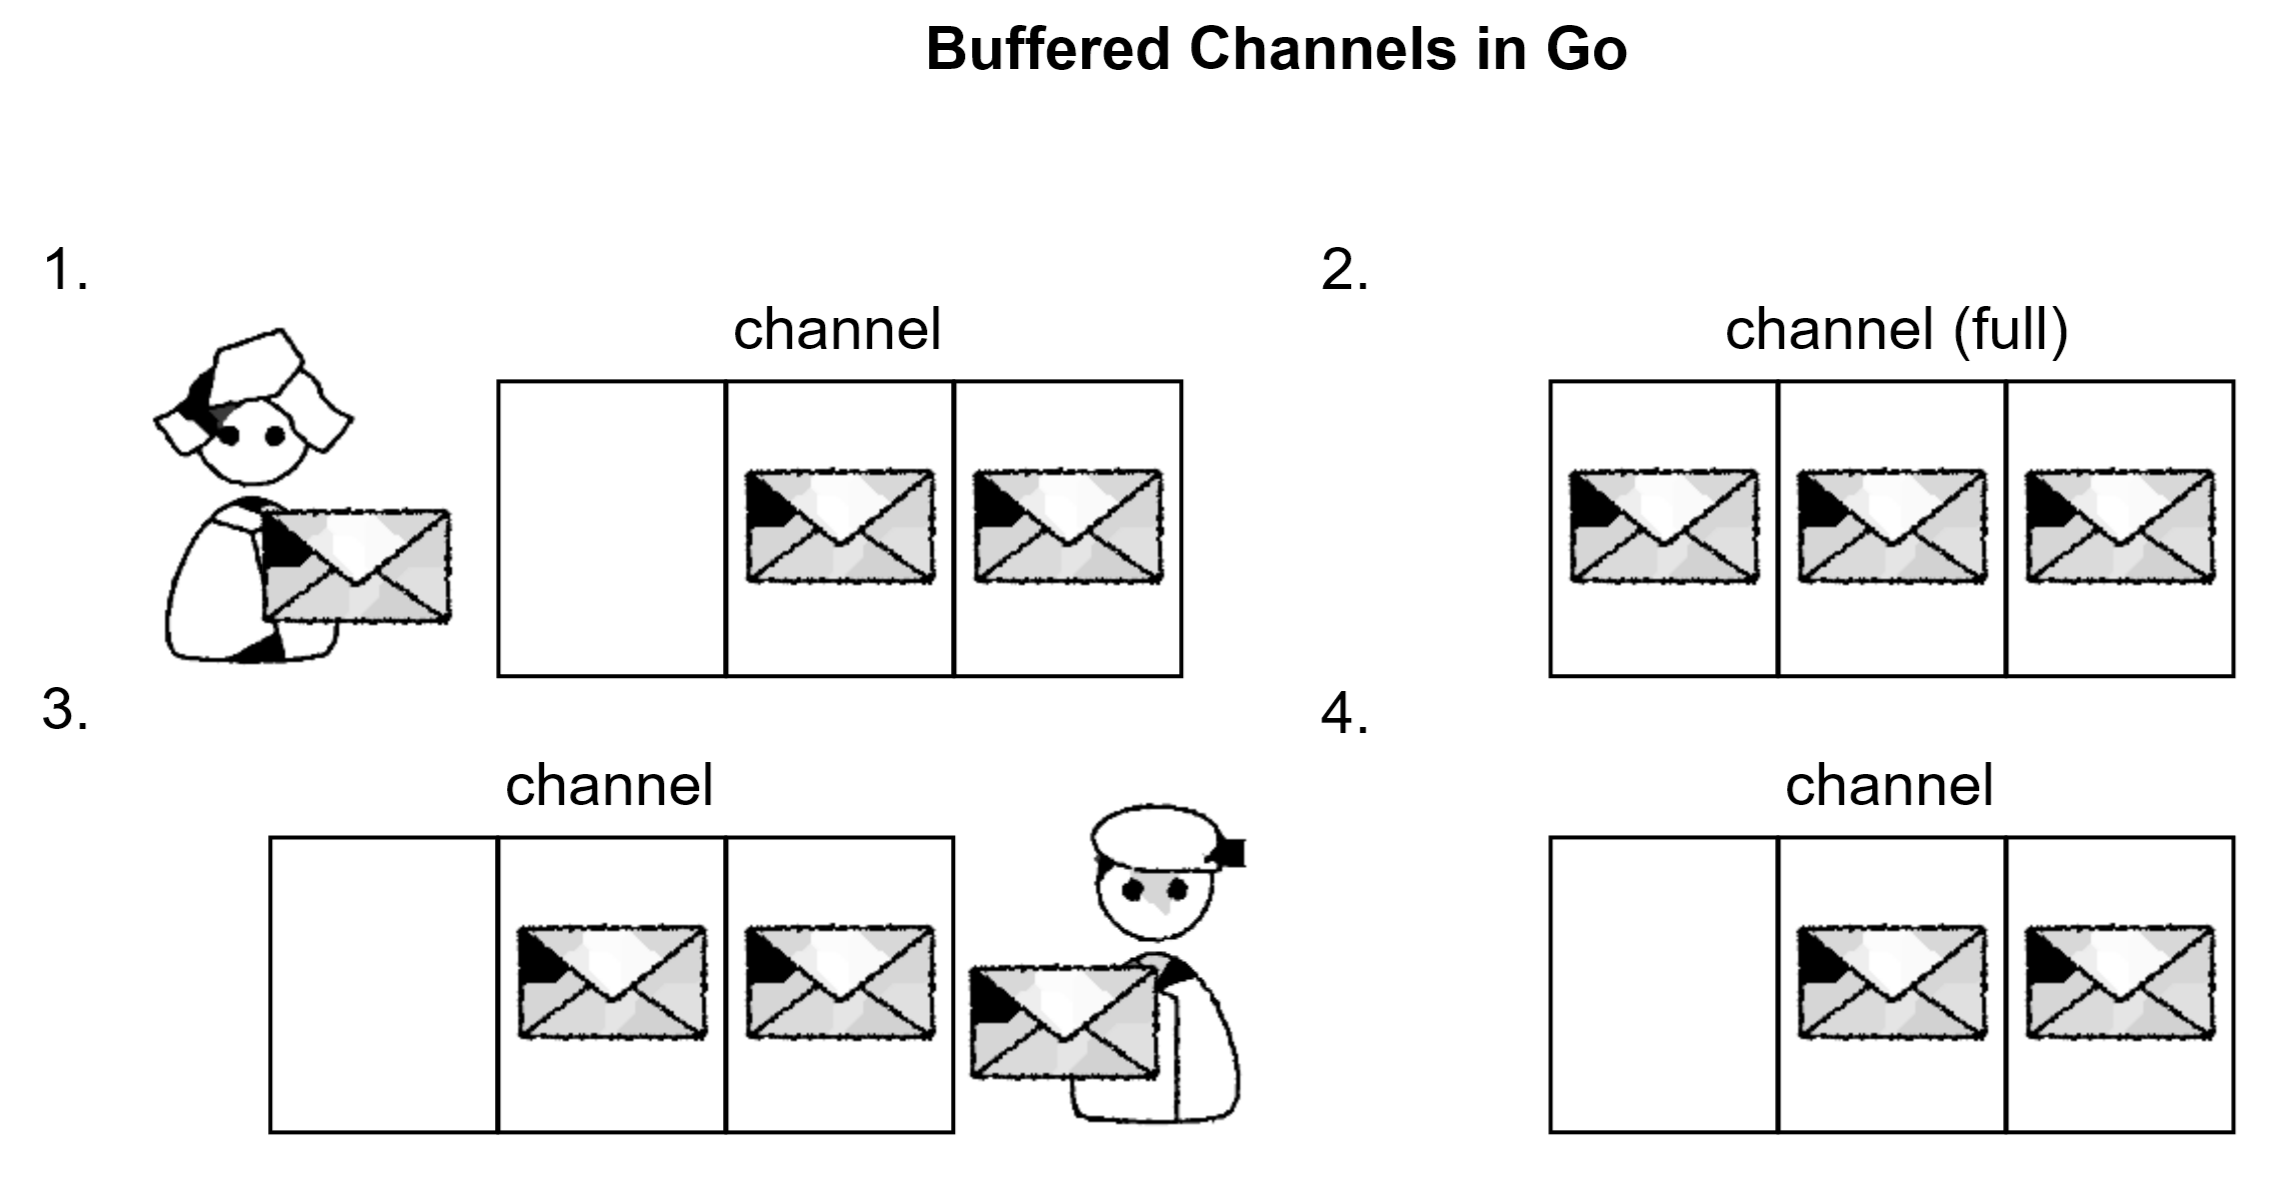
\includegraphics[width=1\textwidth]{Sections/rpc/buffered.png}
    \caption{Buffered channel allowing for asynchronous communication.}
    \label{fig:buffered}
\end{figure}

\noindent
(1) Here Alice (left) fills the channel from left to right with messages. (2) The channel is full and Alice is free to continue her operations. (3) Bob (right) takes the rightmost message from the channel. (4) Bob is free to continue his operations, leaving the channel.\\

\noindent
To make the last example (\ref{ex:channels}) use a buffered channel, we can modify the channel creation.

\begin{Example}[Using Buffered Channels]

    \label{ex:buffered}
    Consider the previous example (\ref{ex:channels}) with a buffered channel:
    \begin{lstlisting}[language=Go, caption=Using Buffered Channels to Synchronize Downloading and Processing, label={lst:buffered}, numbers=none]
    ...
    ch := make(chan int, n) // Buffered channel with a capacity of 5
    ...
    \end{lstlisting}
    \noindent
    Here, the channel has a buffer size of n, allowing up to n messages to be stored before the receiver is ready.
\end{Example}